% Created by tikzDevice version 0.6.2-92-0ad2792 on 2013-05-06 20:58:12
% !TEX encoding = UTF-8 Unicode
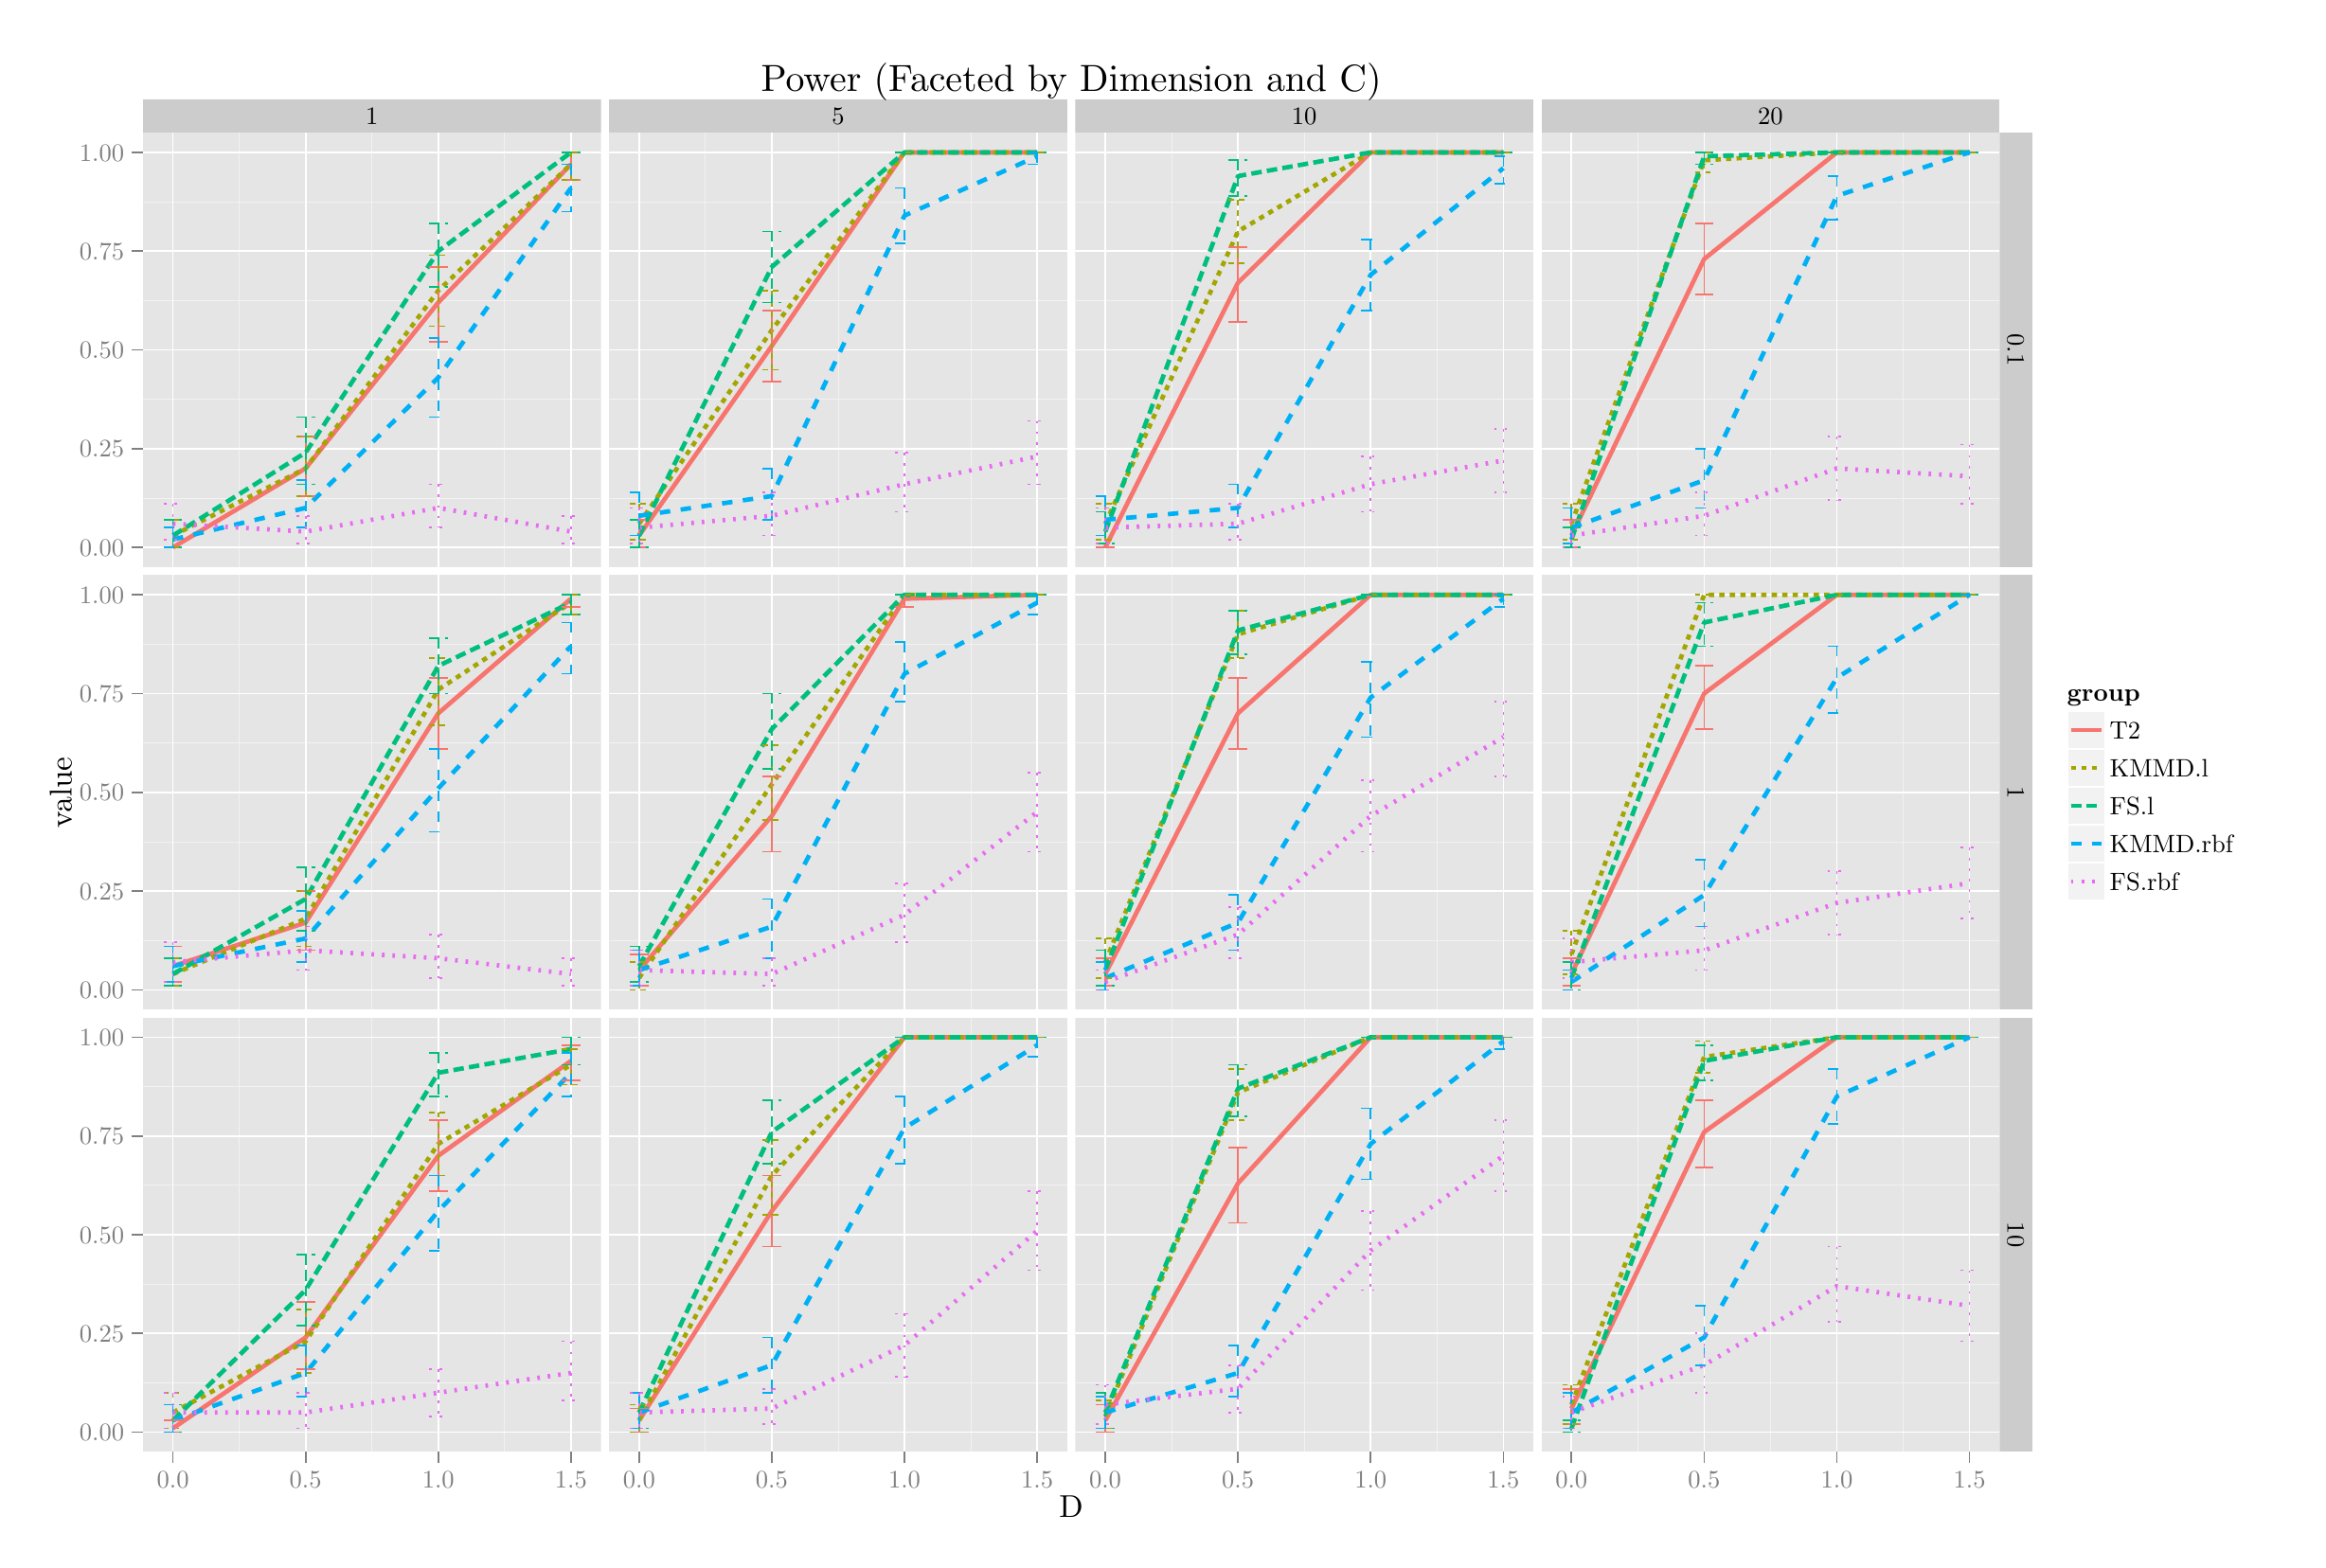
\begin{tikzpicture}[x=1pt,y=1pt]
\definecolor[named]{fillColor}{rgb}{1.00,1.00,1.00}
\path[use as bounding box,fill=fillColor,fill opacity=0.00] (0,0) rectangle (867.24,578.16);
\begin{scope}
\path[clip] (  0.00,  0.00) rectangle (867.24,578.16);
\definecolor[named]{drawColor}{rgb}{1.00,1.00,1.00}
\definecolor[named]{fillColor}{rgb}{1.00,1.00,1.00}

\path[draw=drawColor,line width= 0.6pt,line join=round,line cap=round,fill=fillColor] ( -0.00, -0.00) rectangle (867.24,578.16);
\end{scope}
\begin{scope}
\path[clip] ( 44.49,537.54) rectangle (219.34,550.17);
\definecolor[named]{fillColor}{rgb}{0.80,0.80,0.80}

\path[fill=fillColor] ( 44.49,537.54) rectangle (219.34,550.17);
\definecolor[named]{drawColor}{rgb}{0.00,0.00,0.00}

\node[text=drawColor,anchor=base,inner sep=0pt, outer sep=0pt, scale=  0.96] at (131.91,540.55) {1};
\end{scope}
\begin{scope}
\path[clip] (222.35,537.54) rectangle (397.21,550.17);
\definecolor[named]{fillColor}{rgb}{0.80,0.80,0.80}

\path[fill=fillColor] (222.35,537.54) rectangle (397.21,550.17);
\definecolor[named]{drawColor}{rgb}{0.00,0.00,0.00}

\node[text=drawColor,anchor=base,inner sep=0pt, outer sep=0pt, scale=  0.96] at (309.78,540.55) {5};
\end{scope}
\begin{scope}
\path[clip] (400.22,537.54) rectangle (575.08,550.17);
\definecolor[named]{fillColor}{rgb}{0.80,0.80,0.80}

\path[fill=fillColor] (400.22,537.54) rectangle (575.08,550.17);
\definecolor[named]{drawColor}{rgb}{0.00,0.00,0.00}

\node[text=drawColor,anchor=base,inner sep=0pt, outer sep=0pt, scale=  0.96] at (487.65,540.55) {10};
\end{scope}
\begin{scope}
\path[clip] (578.09,537.54) rectangle (752.95,550.17);
\definecolor[named]{fillColor}{rgb}{0.80,0.80,0.80}

\path[fill=fillColor] (578.09,537.54) rectangle (752.95,550.17);
\definecolor[named]{drawColor}{rgb}{0.00,0.00,0.00}

\node[text=drawColor,anchor=base,inner sep=0pt, outer sep=0pt, scale=  0.96] at (665.52,540.55) {20};
\end{scope}
\begin{scope}
\path[clip] ( 44.49,371.71) rectangle (219.34,537.54);
\definecolor[named]{fillColor}{rgb}{0.90,0.90,0.90}

\path[fill=fillColor] ( 44.49,371.71) rectangle (219.34,537.54);
\definecolor[named]{drawColor}{rgb}{0.95,0.95,0.95}

\path[draw=drawColor,line width= 0.3pt,line join=round] ( 44.49,398.09) --
	(219.34,398.09);

\path[draw=drawColor,line width= 0.3pt,line join=round] ( 44.49,435.78) --
	(219.34,435.78);

\path[draw=drawColor,line width= 0.3pt,line join=round] ( 44.49,473.47) --
	(219.34,473.47);

\path[draw=drawColor,line width= 0.3pt,line join=round] ( 44.49,511.16) --
	(219.34,511.16);

\path[draw=drawColor,line width= 0.3pt,line join=round] ( 81.29,371.71) --
	( 81.29,537.54);

\path[draw=drawColor,line width= 0.3pt,line join=round] (131.91,371.71) --
	(131.91,537.54);

\path[draw=drawColor,line width= 0.3pt,line join=round] (182.54,371.71) --
	(182.54,537.54);
\definecolor[named]{drawColor}{rgb}{1.00,1.00,1.00}

\path[draw=drawColor,line width= 0.6pt,line join=round] ( 44.49,379.25) --
	(219.34,379.25);

\path[draw=drawColor,line width= 0.6pt,line join=round] ( 44.49,416.94) --
	(219.34,416.94);

\path[draw=drawColor,line width= 0.6pt,line join=round] ( 44.49,454.63) --
	(219.34,454.63);

\path[draw=drawColor,line width= 0.6pt,line join=round] ( 44.49,492.31) --
	(219.34,492.31);

\path[draw=drawColor,line width= 0.6pt,line join=round] ( 44.49,530.00) --
	(219.34,530.00);

\path[draw=drawColor,line width= 0.6pt,line join=round] ( 55.98,371.71) --
	( 55.98,537.54);

\path[draw=drawColor,line width= 0.6pt,line join=round] (106.60,371.71) --
	(106.60,537.54);

\path[draw=drawColor,line width= 0.6pt,line join=round] (157.23,371.71) --
	(157.23,537.54);

\path[draw=drawColor,line width= 0.6pt,line join=round] (207.85,371.71) --
	(207.85,537.54);
\definecolor[named]{drawColor}{rgb}{0.97,0.46,0.43}

\path[draw=drawColor,line width= 1.7pt,line join=round] ( 55.98,379.25) --
	(106.60,409.40) --
	(157.23,472.72) --
	(207.85,525.48);
\definecolor[named]{drawColor}{rgb}{0.64,0.65,0.00}

\path[draw=drawColor,line width= 1.7pt,dash pattern=on 2pt off 2pt ,line join=round] ( 55.98,383.77) --
	(106.60,409.40) --
	(157.23,477.24) --
	(207.85,525.48);
\definecolor[named]{drawColor}{rgb}{0.00,0.75,0.49}

\path[draw=drawColor,line width= 1.7pt,dash pattern=on 4pt off 2pt ,line join=round] ( 55.98,383.77) --
	(106.60,415.43) --
	(157.23,492.31) --
	(207.85,530.00);
\definecolor[named]{drawColor}{rgb}{0.00,0.69,0.96}

\path[draw=drawColor,line width= 1.7pt,dash pattern=on 4pt off 4pt ,line join=round] ( 55.98,382.27) --
	(106.60,394.33) --
	(157.23,444.07) --
	(207.85,516.44);
\definecolor[named]{drawColor}{rgb}{0.91,0.42,0.95}

\path[draw=drawColor,line width= 1.7pt,dash pattern=on 1pt off 3pt ,line join=round] ( 55.98,388.30) --
	(106.60,385.28) --
	(157.23,394.33) --
	(207.85,385.28);
\definecolor[named]{drawColor}{rgb}{0.97,0.46,0.43}

\path[draw=drawColor,line width= 0.6pt,line join=round] ( 52.43,379.25) --
	( 59.52,379.25);

\path[draw=drawColor,line width= 0.6pt,line join=round] ( 55.98,379.25) --
	( 55.98,379.25);

\path[draw=drawColor,line width= 0.6pt,line join=round] ( 52.43,379.25) --
	( 59.52,379.25);

\path[draw=drawColor,line width= 0.6pt,line join=round] (103.06,421.46) --
	(110.15,421.46);

\path[draw=drawColor,line width= 0.6pt,line join=round] (106.60,421.46) --
	(106.60,398.85);

\path[draw=drawColor,line width= 0.6pt,line join=round] (103.06,398.85) --
	(110.15,398.85);

\path[draw=drawColor,line width= 0.6pt,line join=round] (153.68,486.28) --
	(160.77,486.28);

\path[draw=drawColor,line width= 0.6pt,line join=round] (157.23,486.28) --
	(157.23,457.64);

\path[draw=drawColor,line width= 0.6pt,line join=round] (153.68,457.64) --
	(160.77,457.64);

\path[draw=drawColor,line width= 0.6pt,line join=round] (204.31,530.00) --
	(211.39,530.00);

\path[draw=drawColor,line width= 0.6pt,line join=round] (207.85,530.00) --
	(207.85,519.45);

\path[draw=drawColor,line width= 0.6pt,line join=round] (204.31,519.45) --
	(211.39,519.45);
\definecolor[named]{drawColor}{rgb}{0.64,0.65,0.00}

\path[draw=drawColor,line width= 0.6pt,dash pattern=on 2pt off 2pt ,line join=round] ( 52.43,389.80) --
	( 59.52,389.80);

\path[draw=drawColor,line width= 0.6pt,dash pattern=on 2pt off 2pt ,line join=round] ( 55.98,389.80) --
	( 55.98,379.25);

\path[draw=drawColor,line width= 0.6pt,dash pattern=on 2pt off 2pt ,line join=round] ( 52.43,379.25) --
	( 59.52,379.25);

\path[draw=drawColor,line width= 0.6pt,dash pattern=on 2pt off 2pt ,line join=round] (103.06,421.46) --
	(110.15,421.46);

\path[draw=drawColor,line width= 0.6pt,dash pattern=on 2pt off 2pt ,line join=round] (106.60,421.46) --
	(106.60,398.81);

\path[draw=drawColor,line width= 0.6pt,dash pattern=on 2pt off 2pt ,line join=round] (103.06,398.81) --
	(110.15,398.81);

\path[draw=drawColor,line width= 0.6pt,dash pattern=on 2pt off 2pt ,line join=round] (153.68,490.81) --
	(160.77,490.81);

\path[draw=drawColor,line width= 0.6pt,dash pattern=on 2pt off 2pt ,line join=round] (157.23,490.81) --
	(157.23,463.63);

\path[draw=drawColor,line width= 0.6pt,dash pattern=on 2pt off 2pt ,line join=round] (153.68,463.63) --
	(160.77,463.63);

\path[draw=drawColor,line width= 0.6pt,dash pattern=on 2pt off 2pt ,line join=round] (204.31,530.00) --
	(211.39,530.00);

\path[draw=drawColor,line width= 0.6pt,dash pattern=on 2pt off 2pt ,line join=round] (207.85,530.00) --
	(207.85,519.45);

\path[draw=drawColor,line width= 0.6pt,dash pattern=on 2pt off 2pt ,line join=round] (204.31,519.45) --
	(211.39,519.45);
\definecolor[named]{drawColor}{rgb}{0.00,0.75,0.49}

\path[draw=drawColor,line width= 0.6pt,dash pattern=on 4pt off 2pt ,line join=round] ( 52.43,389.80) --
	( 59.52,389.80);

\path[draw=drawColor,line width= 0.6pt,dash pattern=on 4pt off 2pt ,line join=round] ( 55.98,389.80) --
	( 55.98,379.25);

\path[draw=drawColor,line width= 0.6pt,dash pattern=on 4pt off 2pt ,line join=round] ( 52.43,379.25) --
	( 59.52,379.25);

\path[draw=drawColor,line width= 0.6pt,dash pattern=on 4pt off 2pt ,line join=round] (103.06,429.00) --
	(110.15,429.00);

\path[draw=drawColor,line width= 0.6pt,dash pattern=on 4pt off 2pt ,line join=round] (106.60,429.00) --
	(106.60,403.37);

\path[draw=drawColor,line width= 0.6pt,dash pattern=on 4pt off 2pt ,line join=round] (103.06,403.37) --
	(110.15,403.37);

\path[draw=drawColor,line width= 0.6pt,dash pattern=on 4pt off 2pt ,line join=round] (153.68,502.87) --
	(160.77,502.87);

\path[draw=drawColor,line width= 0.6pt,dash pattern=on 4pt off 2pt ,line join=round] (157.23,502.87) --
	(157.23,478.75);

\path[draw=drawColor,line width= 0.6pt,dash pattern=on 4pt off 2pt ,line join=round] (153.68,478.75) --
	(160.77,478.75);

\path[draw=drawColor,line width= 0.6pt,dash pattern=on 4pt off 2pt ,line join=round] (204.31,530.00) --
	(211.39,530.00);

\path[draw=drawColor,line width= 0.6pt,dash pattern=on 4pt off 2pt ,line join=round] (207.85,530.00) --
	(207.85,530.00);

\path[draw=drawColor,line width= 0.6pt,dash pattern=on 4pt off 2pt ,line join=round] (204.31,530.00) --
	(211.39,530.00);
\definecolor[named]{drawColor}{rgb}{0.00,0.69,0.96}

\path[draw=drawColor,line width= 0.6pt,dash pattern=on 4pt off 4pt ,line join=round] ( 52.43,386.79) --
	( 59.52,386.79);

\path[draw=drawColor,line width= 0.6pt,dash pattern=on 4pt off 4pt ,line join=round] ( 55.98,386.79) --
	( 55.98,379.25);

\path[draw=drawColor,line width= 0.6pt,dash pattern=on 4pt off 4pt ,line join=round] ( 52.43,379.25) --
	( 59.52,379.25);

\path[draw=drawColor,line width= 0.6pt,dash pattern=on 4pt off 4pt ,line join=round] (103.06,404.88) --
	(110.15,404.88);

\path[draw=drawColor,line width= 0.6pt,dash pattern=on 4pt off 4pt ,line join=round] (106.60,404.88) --
	(106.60,386.79);

\path[draw=drawColor,line width= 0.6pt,dash pattern=on 4pt off 4pt ,line join=round] (103.06,386.79) --
	(110.15,386.79);

\path[draw=drawColor,line width= 0.6pt,dash pattern=on 4pt off 4pt ,line join=round] (153.68,459.15) --
	(160.77,459.15);

\path[draw=drawColor,line width= 0.6pt,dash pattern=on 4pt off 4pt ,line join=round] (157.23,459.15) --
	(157.23,429.00);

\path[draw=drawColor,line width= 0.6pt,dash pattern=on 4pt off 4pt ,line join=round] (153.68,429.00) --
	(160.77,429.00);

\path[draw=drawColor,line width= 0.6pt,dash pattern=on 4pt off 4pt ,line join=round] (204.31,525.48) --
	(211.39,525.48);

\path[draw=drawColor,line width= 0.6pt,dash pattern=on 4pt off 4pt ,line join=round] (207.85,525.48) --
	(207.85,507.39);

\path[draw=drawColor,line width= 0.6pt,dash pattern=on 4pt off 4pt ,line join=round] (204.31,507.39) --
	(211.39,507.39);
\definecolor[named]{drawColor}{rgb}{0.91,0.42,0.95}

\path[draw=drawColor,line width= 0.6pt,dash pattern=on 1pt off 3pt ,line join=round] ( 52.43,395.83) --
	( 59.52,395.83);

\path[draw=drawColor,line width= 0.6pt,dash pattern=on 1pt off 3pt ,line join=round] ( 55.98,395.83) --
	( 55.98,382.27);

\path[draw=drawColor,line width= 0.6pt,dash pattern=on 1pt off 3pt ,line join=round] ( 52.43,382.27) --
	( 59.52,382.27);

\path[draw=drawColor,line width= 0.6pt,dash pattern=on 1pt off 3pt ,line join=round] (103.06,391.31) --
	(110.15,391.31);

\path[draw=drawColor,line width= 0.6pt,dash pattern=on 1pt off 3pt ,line join=round] (106.60,391.31) --
	(106.60,380.76);

\path[draw=drawColor,line width= 0.6pt,dash pattern=on 1pt off 3pt ,line join=round] (103.06,380.76) --
	(110.15,380.76);

\path[draw=drawColor,line width= 0.6pt,dash pattern=on 1pt off 3pt ,line join=round] (153.68,403.37) --
	(160.77,403.37);

\path[draw=drawColor,line width= 0.6pt,dash pattern=on 1pt off 3pt ,line join=round] (157.23,403.37) --
	(157.23,386.79);

\path[draw=drawColor,line width= 0.6pt,dash pattern=on 1pt off 3pt ,line join=round] (153.68,386.79) --
	(160.77,386.79);

\path[draw=drawColor,line width= 0.6pt,dash pattern=on 1pt off 3pt ,line join=round] (204.31,391.31) --
	(211.39,391.31);

\path[draw=drawColor,line width= 0.6pt,dash pattern=on 1pt off 3pt ,line join=round] (207.85,391.31) --
	(207.85,380.76);

\path[draw=drawColor,line width= 0.6pt,dash pattern=on 1pt off 3pt ,line join=round] (204.31,380.76) --
	(211.39,380.76);
\end{scope}
\begin{scope}
\path[clip] ( 44.49,202.87) rectangle (219.34,368.70);
\definecolor[named]{fillColor}{rgb}{0.90,0.90,0.90}

\path[fill=fillColor] ( 44.49,202.87) rectangle (219.34,368.70);
\definecolor[named]{drawColor}{rgb}{0.95,0.95,0.95}

\path[draw=drawColor,line width= 0.3pt,line join=round] ( 44.49,229.26) --
	(219.34,229.26);

\path[draw=drawColor,line width= 0.3pt,line join=round] ( 44.49,266.94) --
	(219.34,266.94);

\path[draw=drawColor,line width= 0.3pt,line join=round] ( 44.49,304.63) --
	(219.34,304.63);

\path[draw=drawColor,line width= 0.3pt,line join=round] ( 44.49,342.32) --
	(219.34,342.32);

\path[draw=drawColor,line width= 0.3pt,line join=round] ( 81.29,202.87) --
	( 81.29,368.70);

\path[draw=drawColor,line width= 0.3pt,line join=round] (131.91,202.87) --
	(131.91,368.70);

\path[draw=drawColor,line width= 0.3pt,line join=round] (182.54,202.87) --
	(182.54,368.70);
\definecolor[named]{drawColor}{rgb}{1.00,1.00,1.00}

\path[draw=drawColor,line width= 0.6pt,line join=round] ( 44.49,210.41) --
	(219.34,210.41);

\path[draw=drawColor,line width= 0.6pt,line join=round] ( 44.49,248.10) --
	(219.34,248.10);

\path[draw=drawColor,line width= 0.6pt,line join=round] ( 44.49,285.79) --
	(219.34,285.79);

\path[draw=drawColor,line width= 0.6pt,line join=round] ( 44.49,323.48) --
	(219.34,323.48);

\path[draw=drawColor,line width= 0.6pt,line join=round] ( 44.49,361.16) --
	(219.34,361.16);

\path[draw=drawColor,line width= 0.6pt,line join=round] ( 55.98,202.87) --
	( 55.98,368.70);

\path[draw=drawColor,line width= 0.6pt,line join=round] (106.60,202.87) --
	(106.60,368.70);

\path[draw=drawColor,line width= 0.6pt,line join=round] (157.23,202.87) --
	(157.23,368.70);

\path[draw=drawColor,line width= 0.6pt,line join=round] (207.85,202.87) --
	(207.85,368.70);
\definecolor[named]{drawColor}{rgb}{0.97,0.46,0.43}

\path[draw=drawColor,line width= 1.7pt,line join=round] ( 55.98,219.46) --
	(106.60,236.04) --
	(157.23,315.94) --
	(207.85,359.66);
\definecolor[named]{drawColor}{rgb}{0.64,0.65,0.00}

\path[draw=drawColor,line width= 1.7pt,dash pattern=on 2pt off 2pt ,line join=round] ( 55.98,216.44) --
	(106.60,237.55) --
	(157.23,324.98) --
	(207.85,358.15);
\definecolor[named]{drawColor}{rgb}{0.00,0.75,0.49}

\path[draw=drawColor,line width= 1.7pt,dash pattern=on 4pt off 2pt ,line join=round] ( 55.98,216.44) --
	(106.60,245.08) --
	(157.23,334.03) --
	(207.85,358.15);
\definecolor[named]{drawColor}{rgb}{0.00,0.69,0.96}

\path[draw=drawColor,line width= 1.7pt,dash pattern=on 4pt off 4pt ,line join=round] ( 55.98,219.46) --
	(106.60,230.01) --
	(157.23,287.30) --
	(207.85,341.57);
\definecolor[named]{drawColor}{rgb}{0.91,0.42,0.95}

\path[draw=drawColor,line width= 1.7pt,dash pattern=on 1pt off 3pt ,line join=round] ( 55.98,220.96) --
	(106.60,225.49) --
	(157.23,222.47) --
	(207.85,216.44);
\definecolor[named]{drawColor}{rgb}{0.97,0.46,0.43}

\path[draw=drawColor,line width= 0.6pt,line join=round] ( 52.43,226.99) --
	( 59.52,226.99);

\path[draw=drawColor,line width= 0.6pt,line join=round] ( 55.98,226.99) --
	( 55.98,213.43);

\path[draw=drawColor,line width= 0.6pt,line join=round] ( 52.43,213.43) --
	( 59.52,213.43);

\path[draw=drawColor,line width= 0.6pt,line join=round] (103.06,248.10) --
	(110.15,248.10);

\path[draw=drawColor,line width= 0.6pt,line join=round] (106.60,248.10) --
	(106.60,225.49);

\path[draw=drawColor,line width= 0.6pt,line join=round] (103.06,225.49) --
	(110.15,225.49);

\path[draw=drawColor,line width= 0.6pt,line join=round] (153.68,329.51) --
	(160.77,329.51);

\path[draw=drawColor,line width= 0.6pt,line join=round] (157.23,329.51) --
	(157.23,302.37);

\path[draw=drawColor,line width= 0.6pt,line join=round] (153.68,302.37) --
	(160.77,302.37);

\path[draw=drawColor,line width= 0.6pt,line join=round] (204.31,361.16) --
	(211.39,361.16);

\path[draw=drawColor,line width= 0.6pt,line join=round] (207.85,361.16) --
	(207.85,356.64);

\path[draw=drawColor,line width= 0.6pt,line join=round] (204.31,356.64) --
	(211.39,356.64);
\definecolor[named]{drawColor}{rgb}{0.64,0.65,0.00}

\path[draw=drawColor,line width= 0.6pt,dash pattern=on 2pt off 2pt ,line join=round] ( 52.43,222.47) --
	( 59.52,222.47);

\path[draw=drawColor,line width= 0.6pt,dash pattern=on 2pt off 2pt ,line join=round] ( 55.98,222.47) --
	( 55.98,211.92);

\path[draw=drawColor,line width= 0.6pt,dash pattern=on 2pt off 2pt ,line join=round] ( 52.43,211.92) --
	( 59.52,211.92);

\path[draw=drawColor,line width= 0.6pt,dash pattern=on 2pt off 2pt ,line join=round] (103.06,248.10) --
	(110.15,248.10);

\path[draw=drawColor,line width= 0.6pt,dash pattern=on 2pt off 2pt ,line join=round] (106.60,248.10) --
	(106.60,226.96);

\path[draw=drawColor,line width= 0.6pt,dash pattern=on 2pt off 2pt ,line join=round] (103.06,226.96) --
	(110.15,226.96);

\path[draw=drawColor,line width= 0.6pt,dash pattern=on 2pt off 2pt ,line join=round] (153.68,337.04) --
	(160.77,337.04);

\path[draw=drawColor,line width= 0.6pt,dash pattern=on 2pt off 2pt ,line join=round] (157.23,337.04) --
	(157.23,311.42);

\path[draw=drawColor,line width= 0.6pt,dash pattern=on 2pt off 2pt ,line join=round] (153.68,311.42) --
	(160.77,311.42);

\path[draw=drawColor,line width= 0.6pt,dash pattern=on 2pt off 2pt ,line join=round] (204.31,361.16) --
	(211.39,361.16);

\path[draw=drawColor,line width= 0.6pt,dash pattern=on 2pt off 2pt ,line join=round] (207.85,361.16) --
	(207.85,353.63);

\path[draw=drawColor,line width= 0.6pt,dash pattern=on 2pt off 2pt ,line join=round] (204.31,353.63) --
	(211.39,353.63);
\definecolor[named]{drawColor}{rgb}{0.00,0.75,0.49}

\path[draw=drawColor,line width= 0.6pt,dash pattern=on 4pt off 2pt ,line join=round] ( 52.43,222.47) --
	( 59.52,222.47);

\path[draw=drawColor,line width= 0.6pt,dash pattern=on 4pt off 2pt ,line join=round] ( 55.98,222.47) --
	( 55.98,211.92);

\path[draw=drawColor,line width= 0.6pt,dash pattern=on 4pt off 2pt ,line join=round] ( 52.43,211.92) --
	( 59.52,211.92);

\path[draw=drawColor,line width= 0.6pt,dash pattern=on 4pt off 2pt ,line join=round] (103.06,257.14) --
	(110.15,257.14);

\path[draw=drawColor,line width= 0.6pt,dash pattern=on 4pt off 2pt ,line join=round] (106.60,257.14) --
	(106.60,233.02);

\path[draw=drawColor,line width= 0.6pt,dash pattern=on 4pt off 2pt ,line join=round] (103.06,233.02) --
	(110.15,233.02);

\path[draw=drawColor,line width= 0.6pt,dash pattern=on 4pt off 2pt ,line join=round] (153.68,344.58) --
	(160.77,344.58);

\path[draw=drawColor,line width= 0.6pt,dash pattern=on 4pt off 2pt ,line join=round] (157.23,344.58) --
	(157.23,323.48);

\path[draw=drawColor,line width= 0.6pt,dash pattern=on 4pt off 2pt ,line join=round] (153.68,323.48) --
	(160.77,323.48);

\path[draw=drawColor,line width= 0.6pt,dash pattern=on 4pt off 2pt ,line join=round] (204.31,361.16) --
	(211.39,361.16);

\path[draw=drawColor,line width= 0.6pt,dash pattern=on 4pt off 2pt ,line join=round] (207.85,361.16) --
	(207.85,353.63);

\path[draw=drawColor,line width= 0.6pt,dash pattern=on 4pt off 2pt ,line join=round] (204.31,353.63) --
	(211.39,353.63);
\definecolor[named]{drawColor}{rgb}{0.00,0.69,0.96}

\path[draw=drawColor,line width= 0.6pt,dash pattern=on 4pt off 4pt ,line join=round] ( 52.43,226.99) --
	( 59.52,226.99);

\path[draw=drawColor,line width= 0.6pt,dash pattern=on 4pt off 4pt ,line join=round] ( 55.98,226.99) --
	( 55.98,213.43);

\path[draw=drawColor,line width= 0.6pt,dash pattern=on 4pt off 4pt ,line join=round] ( 52.43,213.43) --
	( 59.52,213.43);

\path[draw=drawColor,line width= 0.6pt,dash pattern=on 4pt off 4pt ,line join=round] (103.06,240.60) --
	(110.15,240.60);

\path[draw=drawColor,line width= 0.6pt,dash pattern=on 4pt off 4pt ,line join=round] (106.60,240.60) --
	(106.60,220.96);

\path[draw=drawColor,line width= 0.6pt,dash pattern=on 4pt off 4pt ,line join=round] (103.06,220.96) --
	(110.15,220.96);

\path[draw=drawColor,line width= 0.6pt,dash pattern=on 4pt off 4pt ,line join=round] (153.68,302.37) --
	(160.77,302.37);

\path[draw=drawColor,line width= 0.6pt,dash pattern=on 4pt off 4pt ,line join=round] (157.23,302.37) --
	(157.23,270.71);

\path[draw=drawColor,line width= 0.6pt,dash pattern=on 4pt off 4pt ,line join=round] (153.68,270.71) --
	(160.77,270.71);

\path[draw=drawColor,line width= 0.6pt,dash pattern=on 4pt off 4pt ,line join=round] (204.31,350.61) --
	(211.39,350.61);

\path[draw=drawColor,line width= 0.6pt,dash pattern=on 4pt off 4pt ,line join=round] (207.85,350.61) --
	(207.85,331.01);

\path[draw=drawColor,line width= 0.6pt,dash pattern=on 4pt off 4pt ,line join=round] (204.31,331.01) --
	(211.39,331.01);
\definecolor[named]{drawColor}{rgb}{0.91,0.42,0.95}

\path[draw=drawColor,line width= 0.6pt,dash pattern=on 1pt off 3pt ,line join=round] ( 52.43,228.50) --
	( 59.52,228.50);

\path[draw=drawColor,line width= 0.6pt,dash pattern=on 1pt off 3pt ,line join=round] ( 55.98,228.50) --
	( 55.98,213.43);

\path[draw=drawColor,line width= 0.6pt,dash pattern=on 1pt off 3pt ,line join=round] ( 52.43,213.43) --
	( 59.52,213.43);

\path[draw=drawColor,line width= 0.6pt,dash pattern=on 1pt off 3pt ,line join=round] (103.06,234.53) --
	(110.15,234.53);

\path[draw=drawColor,line width= 0.6pt,dash pattern=on 1pt off 3pt ,line join=round] (106.60,234.53) --
	(106.60,217.95);

\path[draw=drawColor,line width= 0.6pt,dash pattern=on 1pt off 3pt ,line join=round] (103.06,217.95) --
	(110.15,217.95);

\path[draw=drawColor,line width= 0.6pt,dash pattern=on 1pt off 3pt ,line join=round] (153.68,231.52) --
	(160.77,231.52);

\path[draw=drawColor,line width= 0.6pt,dash pattern=on 1pt off 3pt ,line join=round] (157.23,231.52) --
	(157.23,214.93);

\path[draw=drawColor,line width= 0.6pt,dash pattern=on 1pt off 3pt ,line join=round] (153.68,214.93) --
	(160.77,214.93);

\path[draw=drawColor,line width= 0.6pt,dash pattern=on 1pt off 3pt ,line join=round] (204.31,222.47) --
	(211.39,222.47);

\path[draw=drawColor,line width= 0.6pt,dash pattern=on 1pt off 3pt ,line join=round] (207.85,222.47) --
	(207.85,211.92);

\path[draw=drawColor,line width= 0.6pt,dash pattern=on 1pt off 3pt ,line join=round] (204.31,211.92) --
	(211.39,211.92);
\end{scope}
\begin{scope}
\path[clip] ( 44.49, 34.03) rectangle (219.34,199.86);
\definecolor[named]{fillColor}{rgb}{0.90,0.90,0.90}

\path[fill=fillColor] ( 44.49, 34.03) rectangle (219.34,199.86);
\definecolor[named]{drawColor}{rgb}{0.95,0.95,0.95}

\path[draw=drawColor,line width= 0.3pt,line join=round] ( 44.49, 60.42) --
	(219.34, 60.42);

\path[draw=drawColor,line width= 0.3pt,line join=round] ( 44.49, 98.10) --
	(219.34, 98.10);

\path[draw=drawColor,line width= 0.3pt,line join=round] ( 44.49,135.79) --
	(219.34,135.79);

\path[draw=drawColor,line width= 0.3pt,line join=round] ( 44.49,173.48) --
	(219.34,173.48);

\path[draw=drawColor,line width= 0.3pt,line join=round] ( 81.29, 34.03) --
	( 81.29,199.86);

\path[draw=drawColor,line width= 0.3pt,line join=round] (131.91, 34.03) --
	(131.91,199.86);

\path[draw=drawColor,line width= 0.3pt,line join=round] (182.54, 34.03) --
	(182.54,199.86);
\definecolor[named]{drawColor}{rgb}{1.00,1.00,1.00}

\path[draw=drawColor,line width= 0.6pt,line join=round] ( 44.49, 41.57) --
	(219.34, 41.57);

\path[draw=drawColor,line width= 0.6pt,line join=round] ( 44.49, 79.26) --
	(219.34, 79.26);

\path[draw=drawColor,line width= 0.6pt,line join=round] ( 44.49,116.95) --
	(219.34,116.95);

\path[draw=drawColor,line width= 0.6pt,line join=round] ( 44.49,154.64) --
	(219.34,154.64);

\path[draw=drawColor,line width= 0.6pt,line join=round] ( 44.49,192.32) --
	(219.34,192.32);

\path[draw=drawColor,line width= 0.6pt,line join=round] ( 55.98, 34.03) --
	( 55.98,199.86);

\path[draw=drawColor,line width= 0.6pt,line join=round] (106.60, 34.03) --
	(106.60,199.86);

\path[draw=drawColor,line width= 0.6pt,line join=round] (157.23, 34.03) --
	(157.23,199.86);

\path[draw=drawColor,line width= 0.6pt,line join=round] (207.85, 34.03) --
	(207.85,199.86);
\definecolor[named]{drawColor}{rgb}{0.97,0.46,0.43}

\path[draw=drawColor,line width= 1.7pt,line join=round] ( 55.98, 43.08) --
	(106.60, 77.75) --
	(157.23,147.10) --
	(207.85,183.28);
\definecolor[named]{drawColor}{rgb}{0.64,0.65,0.00}

\path[draw=drawColor,line width= 1.7pt,dash pattern=on 2pt off 2pt ,line join=round] ( 55.98, 49.11) --
	(106.60, 76.25) --
	(157.23,151.62) --
	(207.85,181.77);
\definecolor[named]{drawColor}{rgb}{0.00,0.75,0.49}

\path[draw=drawColor,line width= 1.7pt,dash pattern=on 4pt off 2pt ,line join=round] ( 55.98, 46.09) --
	(106.60, 95.84) --
	(157.23,178.76) --
	(207.85,187.80);
\definecolor[named]{drawColor}{rgb}{0.00,0.69,0.96}

\path[draw=drawColor,line width= 1.7pt,dash pattern=on 4pt off 4pt ,line join=round] ( 55.98, 46.09) --
	(106.60, 64.19) --
	(157.23,125.99) --
	(207.85,178.76);
\definecolor[named]{drawColor}{rgb}{0.91,0.42,0.95}

\path[draw=drawColor,line width= 1.7pt,dash pattern=on 1pt off 3pt ,line join=round] ( 55.98, 49.11) --
	(106.60, 49.11) --
	(157.23, 56.65) --
	(207.85, 64.19);
\definecolor[named]{drawColor}{rgb}{0.97,0.46,0.43}

\path[draw=drawColor,line width= 0.6pt,line join=round] ( 52.43, 46.09) --
	( 59.52, 46.09);

\path[draw=drawColor,line width= 0.6pt,line join=round] ( 55.98, 46.09) --
	( 55.98, 41.57);

\path[draw=drawColor,line width= 0.6pt,line join=round] ( 52.43, 41.57) --
	( 59.52, 41.57);

\path[draw=drawColor,line width= 0.6pt,line join=round] (103.06, 91.32) --
	(110.15, 91.32);

\path[draw=drawColor,line width= 0.6pt,line join=round] (106.60, 91.32) --
	(106.60, 65.69);

\path[draw=drawColor,line width= 0.6pt,line join=round] (103.06, 65.69) --
	(110.15, 65.69);

\path[draw=drawColor,line width= 0.6pt,line join=round] (153.68,160.67) --
	(160.77,160.67);

\path[draw=drawColor,line width= 0.6pt,line join=round] (157.23,160.67) --
	(157.23,133.53);

\path[draw=drawColor,line width= 0.6pt,line join=round] (153.68,133.53) --
	(160.77,133.53);

\path[draw=drawColor,line width= 0.6pt,line join=round] (204.31,189.31) --
	(211.39,189.31);

\path[draw=drawColor,line width= 0.6pt,line join=round] (207.85,189.31) --
	(207.85,175.74);

\path[draw=drawColor,line width= 0.6pt,line join=round] (204.31,175.74) --
	(211.39,175.74);
\definecolor[named]{drawColor}{rgb}{0.64,0.65,0.00}

\path[draw=drawColor,line width= 0.6pt,dash pattern=on 2pt off 2pt ,line join=round] ( 52.43, 56.65) --
	( 59.52, 56.65);

\path[draw=drawColor,line width= 0.6pt,dash pattern=on 2pt off 2pt ,line join=round] ( 55.98, 56.65) --
	( 55.98, 43.08);

\path[draw=drawColor,line width= 0.6pt,dash pattern=on 2pt off 2pt ,line join=round] ( 52.43, 43.08) --
	( 59.52, 43.08);

\path[draw=drawColor,line width= 0.6pt,dash pattern=on 2pt off 2pt ,line join=round] (103.06, 88.31) --
	(110.15, 88.31);

\path[draw=drawColor,line width= 0.6pt,dash pattern=on 2pt off 2pt ,line join=round] (106.60, 88.31) --
	(106.60, 64.19);

\path[draw=drawColor,line width= 0.6pt,dash pattern=on 2pt off 2pt ,line join=round] (103.06, 64.19) --
	(110.15, 64.19);

\path[draw=drawColor,line width= 0.6pt,dash pattern=on 2pt off 2pt ,line join=round] (153.68,163.68) --
	(160.77,163.68);

\path[draw=drawColor,line width= 0.6pt,dash pattern=on 2pt off 2pt ,line join=round] (157.23,163.68) --
	(157.23,139.56);

\path[draw=drawColor,line width= 0.6pt,dash pattern=on 2pt off 2pt ,line join=round] (153.68,139.56) --
	(160.77,139.56);

\path[draw=drawColor,line width= 0.6pt,dash pattern=on 2pt off 2pt ,line join=round] (204.31,187.80) --
	(211.39,187.80);

\path[draw=drawColor,line width= 0.6pt,dash pattern=on 2pt off 2pt ,line join=round] (207.85,187.80) --
	(207.85,174.23);

\path[draw=drawColor,line width= 0.6pt,dash pattern=on 2pt off 2pt ,line join=round] (204.31,174.23) --
	(211.39,174.23);
\definecolor[named]{drawColor}{rgb}{0.00,0.75,0.49}

\path[draw=drawColor,line width= 0.6pt,dash pattern=on 4pt off 2pt ,line join=round] ( 52.43, 52.12) --
	( 59.52, 52.12);

\path[draw=drawColor,line width= 0.6pt,dash pattern=on 4pt off 2pt ,line join=round] ( 55.98, 52.12) --
	( 55.98, 41.57);

\path[draw=drawColor,line width= 0.6pt,dash pattern=on 4pt off 2pt ,line join=round] ( 52.43, 41.57) --
	( 59.52, 41.57);

\path[draw=drawColor,line width= 0.6pt,dash pattern=on 4pt off 2pt ,line join=round] (103.06,109.41) --
	(110.15,109.41);

\path[draw=drawColor,line width= 0.6pt,dash pattern=on 4pt off 2pt ,line join=round] (106.60,109.41) --
	(106.60, 82.28);

\path[draw=drawColor,line width= 0.6pt,dash pattern=on 4pt off 2pt ,line join=round] (103.06, 82.28) --
	(110.15, 82.28);

\path[draw=drawColor,line width= 0.6pt,dash pattern=on 4pt off 2pt ,line join=round] (153.68,186.29) --
	(160.77,186.29);

\path[draw=drawColor,line width= 0.6pt,dash pattern=on 4pt off 2pt ,line join=round] (157.23,186.29) --
	(157.23,169.71);

\path[draw=drawColor,line width= 0.6pt,dash pattern=on 4pt off 2pt ,line join=round] (153.68,169.71) --
	(160.77,169.71);

\path[draw=drawColor,line width= 0.6pt,dash pattern=on 4pt off 2pt ,line join=round] (204.31,192.32) --
	(211.39,192.32);

\path[draw=drawColor,line width= 0.6pt,dash pattern=on 4pt off 2pt ,line join=round] (207.85,192.32) --
	(207.85,181.77);

\path[draw=drawColor,line width= 0.6pt,dash pattern=on 4pt off 2pt ,line join=round] (204.31,181.77) --
	(211.39,181.77);
\definecolor[named]{drawColor}{rgb}{0.00,0.69,0.96}

\path[draw=drawColor,line width= 0.6pt,dash pattern=on 4pt off 4pt ,line join=round] ( 52.43, 52.12) --
	( 59.52, 52.12);

\path[draw=drawColor,line width= 0.6pt,dash pattern=on 4pt off 4pt ,line join=round] ( 55.98, 52.12) --
	( 55.98, 41.57);

\path[draw=drawColor,line width= 0.6pt,dash pattern=on 4pt off 4pt ,line join=round] ( 52.43, 41.57) --
	( 59.52, 41.57);

\path[draw=drawColor,line width= 0.6pt,dash pattern=on 4pt off 4pt ,line join=round] (103.06, 74.78) --
	(110.15, 74.78);

\path[draw=drawColor,line width= 0.6pt,dash pattern=on 4pt off 4pt ,line join=round] (106.60, 74.78) --
	(106.60, 55.14);

\path[draw=drawColor,line width= 0.6pt,dash pattern=on 4pt off 4pt ,line join=round] (103.06, 55.14) --
	(110.15, 55.14);

\path[draw=drawColor,line width= 0.6pt,dash pattern=on 4pt off 4pt ,line join=round] (153.68,139.56) --
	(160.77,139.56);

\path[draw=drawColor,line width= 0.6pt,dash pattern=on 4pt off 4pt ,line join=round] (157.23,139.56) --
	(157.23,110.92);

\path[draw=drawColor,line width= 0.6pt,dash pattern=on 4pt off 4pt ,line join=round] (153.68,110.92) --
	(160.77,110.92);

\path[draw=drawColor,line width= 0.6pt,dash pattern=on 4pt off 4pt ,line join=round] (204.31,186.29) --
	(211.39,186.29);

\path[draw=drawColor,line width= 0.6pt,dash pattern=on 4pt off 4pt ,line join=round] (207.85,186.29) --
	(207.85,169.71);

\path[draw=drawColor,line width= 0.6pt,dash pattern=on 4pt off 4pt ,line join=round] (204.31,169.71) --
	(211.39,169.71);
\definecolor[named]{drawColor}{rgb}{0.91,0.42,0.95}

\path[draw=drawColor,line width= 0.6pt,dash pattern=on 1pt off 3pt ,line join=round] ( 52.43, 56.65) --
	( 59.52, 56.65);

\path[draw=drawColor,line width= 0.6pt,dash pattern=on 1pt off 3pt ,line join=round] ( 55.98, 56.65) --
	( 55.98, 43.08);

\path[draw=drawColor,line width= 0.6pt,dash pattern=on 1pt off 3pt ,line join=round] ( 52.43, 43.08) --
	( 59.52, 43.08);

\path[draw=drawColor,line width= 0.6pt,dash pattern=on 1pt off 3pt ,line join=round] (103.06, 56.65) --
	(110.15, 56.65);

\path[draw=drawColor,line width= 0.6pt,dash pattern=on 1pt off 3pt ,line join=round] (106.60, 56.65) --
	(106.60, 43.08);

\path[draw=drawColor,line width= 0.6pt,dash pattern=on 1pt off 3pt ,line join=round] (103.06, 43.08) --
	(110.15, 43.08);

\path[draw=drawColor,line width= 0.6pt,dash pattern=on 1pt off 3pt ,line join=round] (153.68, 65.69) --
	(160.77, 65.69);

\path[draw=drawColor,line width= 0.6pt,dash pattern=on 1pt off 3pt ,line join=round] (157.23, 65.69) --
	(157.23, 47.60);

\path[draw=drawColor,line width= 0.6pt,dash pattern=on 1pt off 3pt ,line join=round] (153.68, 47.60) --
	(160.77, 47.60);

\path[draw=drawColor,line width= 0.6pt,dash pattern=on 1pt off 3pt ,line join=round] (204.31, 76.25) --
	(211.39, 76.25);

\path[draw=drawColor,line width= 0.6pt,dash pattern=on 1pt off 3pt ,line join=round] (207.85, 76.25) --
	(207.85, 53.63);

\path[draw=drawColor,line width= 0.6pt,dash pattern=on 1pt off 3pt ,line join=round] (204.31, 53.63) --
	(211.39, 53.63);
\end{scope}
\begin{scope}
\path[clip] (222.35,371.71) rectangle (397.21,537.54);
\definecolor[named]{fillColor}{rgb}{0.90,0.90,0.90}

\path[fill=fillColor] (222.35,371.71) rectangle (397.21,537.54);
\definecolor[named]{drawColor}{rgb}{0.95,0.95,0.95}

\path[draw=drawColor,line width= 0.3pt,line join=round] (222.35,398.09) --
	(397.21,398.09);

\path[draw=drawColor,line width= 0.3pt,line join=round] (222.35,435.78) --
	(397.21,435.78);

\path[draw=drawColor,line width= 0.3pt,line join=round] (222.35,473.47) --
	(397.21,473.47);

\path[draw=drawColor,line width= 0.3pt,line join=round] (222.35,511.16) --
	(397.21,511.16);

\path[draw=drawColor,line width= 0.3pt,line join=round] (259.16,371.71) --
	(259.16,537.54);

\path[draw=drawColor,line width= 0.3pt,line join=round] (309.78,371.71) --
	(309.78,537.54);

\path[draw=drawColor,line width= 0.3pt,line join=round] (360.41,371.71) --
	(360.41,537.54);
\definecolor[named]{drawColor}{rgb}{1.00,1.00,1.00}

\path[draw=drawColor,line width= 0.6pt,line join=round] (222.35,379.25) --
	(397.21,379.25);

\path[draw=drawColor,line width= 0.6pt,line join=round] (222.35,416.94) --
	(397.21,416.94);

\path[draw=drawColor,line width= 0.6pt,line join=round] (222.35,454.63) --
	(397.21,454.63);

\path[draw=drawColor,line width= 0.6pt,line join=round] (222.35,492.31) --
	(397.21,492.31);

\path[draw=drawColor,line width= 0.6pt,line join=round] (222.35,530.00) --
	(397.21,530.00);

\path[draw=drawColor,line width= 0.6pt,line join=round] (233.85,371.71) --
	(233.85,537.54);

\path[draw=drawColor,line width= 0.6pt,line join=round] (284.47,371.71) --
	(284.47,537.54);

\path[draw=drawColor,line width= 0.6pt,line join=round] (335.09,371.71) --
	(335.09,537.54);

\path[draw=drawColor,line width= 0.6pt,line join=round] (385.72,371.71) --
	(385.72,537.54);
\definecolor[named]{drawColor}{rgb}{0.97,0.46,0.43}

\path[draw=drawColor,line width= 1.7pt,line join=round] (233.85,383.77) --
	(284.47,456.13) --
	(335.09,530.00) --
	(385.72,530.00);
\definecolor[named]{drawColor}{rgb}{0.64,0.65,0.00}

\path[draw=drawColor,line width= 1.7pt,dash pattern=on 2pt off 2pt ,line join=round] (233.85,388.30) --
	(284.47,462.16) --
	(335.09,530.00) --
	(385.72,530.00);
\definecolor[named]{drawColor}{rgb}{0.00,0.75,0.49}

\path[draw=drawColor,line width= 1.7pt,dash pattern=on 4pt off 2pt ,line join=round] (233.85,383.77) --
	(284.47,486.28) --
	(335.09,530.00) --
	(385.72,530.00);
\definecolor[named]{drawColor}{rgb}{0.00,0.69,0.96}

\path[draw=drawColor,line width= 1.7pt,dash pattern=on 4pt off 4pt ,line join=round] (233.85,391.31) --
	(284.47,398.85) --
	(335.09,505.88) --
	(385.72,528.50);
\definecolor[named]{drawColor}{rgb}{0.91,0.42,0.95}

\path[draw=drawColor,line width= 1.7pt,dash pattern=on 1pt off 3pt ,line join=round] (233.85,386.79) --
	(284.47,391.31) --
	(335.09,403.37) --
	(385.72,413.92);
\definecolor[named]{drawColor}{rgb}{0.97,0.46,0.43}

\path[draw=drawColor,line width= 0.6pt,line join=round] (230.30,389.80) --
	(237.39,389.80);

\path[draw=drawColor,line width= 0.6pt,line join=round] (233.85,389.80) --
	(233.85,379.25);

\path[draw=drawColor,line width= 0.6pt,line join=round] (230.30,379.25) --
	(237.39,379.25);

\path[draw=drawColor,line width= 0.6pt,line join=round] (280.93,469.70) --
	(288.01,469.70);

\path[draw=drawColor,line width= 0.6pt,line join=round] (284.47,469.70) --
	(284.47,442.57);

\path[draw=drawColor,line width= 0.6pt,line join=round] (280.93,442.57) --
	(288.01,442.57);

\path[draw=drawColor,line width= 0.6pt,line join=round] (331.55,530.00) --
	(338.64,530.00);

\path[draw=drawColor,line width= 0.6pt,line join=round] (335.09,530.00) --
	(335.09,530.00);

\path[draw=drawColor,line width= 0.6pt,line join=round] (331.55,530.00) --
	(338.64,530.00);

\path[draw=drawColor,line width= 0.6pt,line join=round] (382.17,530.00) --
	(389.26,530.00);

\path[draw=drawColor,line width= 0.6pt,line join=round] (385.72,530.00) --
	(385.72,530.00);

\path[draw=drawColor,line width= 0.6pt,line join=round] (382.17,530.00) --
	(389.26,530.00);
\definecolor[named]{drawColor}{rgb}{0.64,0.65,0.00}

\path[draw=drawColor,line width= 0.6pt,dash pattern=on 2pt off 2pt ,line join=round] (230.30,395.83) --
	(237.39,395.83);

\path[draw=drawColor,line width= 0.6pt,dash pattern=on 2pt off 2pt ,line join=round] (233.85,395.83) --
	(233.85,382.27);

\path[draw=drawColor,line width= 0.6pt,dash pattern=on 2pt off 2pt ,line join=round] (230.30,382.27) --
	(237.39,382.27);

\path[draw=drawColor,line width= 0.6pt,dash pattern=on 2pt off 2pt ,line join=round] (280.93,477.24) --
	(288.01,477.24);

\path[draw=drawColor,line width= 0.6pt,dash pattern=on 2pt off 2pt ,line join=round] (284.47,477.24) --
	(284.47,447.09);

\path[draw=drawColor,line width= 0.6pt,dash pattern=on 2pt off 2pt ,line join=round] (280.93,447.09) --
	(288.01,447.09);

\path[draw=drawColor,line width= 0.6pt,dash pattern=on 2pt off 2pt ,line join=round] (331.55,530.00) --
	(338.64,530.00);

\path[draw=drawColor,line width= 0.6pt,dash pattern=on 2pt off 2pt ,line join=round] (335.09,530.00) --
	(335.09,530.00);

\path[draw=drawColor,line width= 0.6pt,dash pattern=on 2pt off 2pt ,line join=round] (331.55,530.00) --
	(338.64,530.00);

\path[draw=drawColor,line width= 0.6pt,dash pattern=on 2pt off 2pt ,line join=round] (382.17,530.00) --
	(389.26,530.00);

\path[draw=drawColor,line width= 0.6pt,dash pattern=on 2pt off 2pt ,line join=round] (385.72,530.00) --
	(385.72,530.00);

\path[draw=drawColor,line width= 0.6pt,dash pattern=on 2pt off 2pt ,line join=round] (382.17,530.00) --
	(389.26,530.00);
\definecolor[named]{drawColor}{rgb}{0.00,0.75,0.49}

\path[draw=drawColor,line width= 0.6pt,dash pattern=on 4pt off 2pt ,line join=round] (230.30,389.80) --
	(237.39,389.80);

\path[draw=drawColor,line width= 0.6pt,dash pattern=on 4pt off 2pt ,line join=round] (233.85,389.80) --
	(233.85,379.25);

\path[draw=drawColor,line width= 0.6pt,dash pattern=on 4pt off 2pt ,line join=round] (230.30,379.25) --
	(237.39,379.25);

\path[draw=drawColor,line width= 0.6pt,dash pattern=on 4pt off 2pt ,line join=round] (280.93,499.85) --
	(288.01,499.85);

\path[draw=drawColor,line width= 0.6pt,dash pattern=on 4pt off 2pt ,line join=round] (284.47,499.85) --
	(284.47,472.72);

\path[draw=drawColor,line width= 0.6pt,dash pattern=on 4pt off 2pt ,line join=round] (280.93,472.72) --
	(288.01,472.72);

\path[draw=drawColor,line width= 0.6pt,dash pattern=on 4pt off 2pt ,line join=round] (331.55,530.00) --
	(338.64,530.00);

\path[draw=drawColor,line width= 0.6pt,dash pattern=on 4pt off 2pt ,line join=round] (335.09,530.00) --
	(335.09,530.00);

\path[draw=drawColor,line width= 0.6pt,dash pattern=on 4pt off 2pt ,line join=round] (331.55,530.00) --
	(338.64,530.00);

\path[draw=drawColor,line width= 0.6pt,dash pattern=on 4pt off 2pt ,line join=round] (382.17,530.00) --
	(389.26,530.00);

\path[draw=drawColor,line width= 0.6pt,dash pattern=on 4pt off 2pt ,line join=round] (385.72,530.00) --
	(385.72,530.00);

\path[draw=drawColor,line width= 0.6pt,dash pattern=on 4pt off 2pt ,line join=round] (382.17,530.00) --
	(389.26,530.00);
\definecolor[named]{drawColor}{rgb}{0.00,0.69,0.96}

\path[draw=drawColor,line width= 0.6pt,dash pattern=on 4pt off 4pt ,line join=round] (230.30,400.36) --
	(237.39,400.36);

\path[draw=drawColor,line width= 0.6pt,dash pattern=on 4pt off 4pt ,line join=round] (233.85,400.36) --
	(233.85,383.77);

\path[draw=drawColor,line width= 0.6pt,dash pattern=on 4pt off 4pt ,line join=round] (230.30,383.77) --
	(237.39,383.77);

\path[draw=drawColor,line width= 0.6pt,dash pattern=on 4pt off 4pt ,line join=round] (280.93,409.40) --
	(288.01,409.40);

\path[draw=drawColor,line width= 0.6pt,dash pattern=on 4pt off 4pt ,line join=round] (284.47,409.40) --
	(284.47,389.80);

\path[draw=drawColor,line width= 0.6pt,dash pattern=on 4pt off 4pt ,line join=round] (280.93,389.80) --
	(288.01,389.80);

\path[draw=drawColor,line width= 0.6pt,dash pattern=on 4pt off 4pt ,line join=round] (331.55,516.44) --
	(338.64,516.44);

\path[draw=drawColor,line width= 0.6pt,dash pattern=on 4pt off 4pt ,line join=round] (335.09,516.44) --
	(335.09,495.33);

\path[draw=drawColor,line width= 0.6pt,dash pattern=on 4pt off 4pt ,line join=round] (331.55,495.33) --
	(338.64,495.33);

\path[draw=drawColor,line width= 0.6pt,dash pattern=on 4pt off 4pt ,line join=round] (382.17,530.00) --
	(389.26,530.00);

\path[draw=drawColor,line width= 0.6pt,dash pattern=on 4pt off 4pt ,line join=round] (385.72,530.00) --
	(385.72,525.48);

\path[draw=drawColor,line width= 0.6pt,dash pattern=on 4pt off 4pt ,line join=round] (382.17,525.48) --
	(389.26,525.48);
\definecolor[named]{drawColor}{rgb}{0.91,0.42,0.95}

\path[draw=drawColor,line width= 0.6pt,dash pattern=on 1pt off 3pt ,line join=round] (230.30,394.33) --
	(237.39,394.33);

\path[draw=drawColor,line width= 0.6pt,dash pattern=on 1pt off 3pt ,line join=round] (233.85,394.33) --
	(233.85,380.76);

\path[draw=drawColor,line width= 0.6pt,dash pattern=on 1pt off 3pt ,line join=round] (230.30,380.76) --
	(237.39,380.76);

\path[draw=drawColor,line width= 0.6pt,dash pattern=on 1pt off 3pt ,line join=round] (280.93,400.36) --
	(288.01,400.36);

\path[draw=drawColor,line width= 0.6pt,dash pattern=on 1pt off 3pt ,line join=round] (284.47,400.36) --
	(284.47,383.77);

\path[draw=drawColor,line width= 0.6pt,dash pattern=on 1pt off 3pt ,line join=round] (280.93,383.77) --
	(288.01,383.77);

\path[draw=drawColor,line width= 0.6pt,dash pattern=on 1pt off 3pt ,line join=round] (331.55,415.43) --
	(338.64,415.43);

\path[draw=drawColor,line width= 0.6pt,dash pattern=on 1pt off 3pt ,line join=round] (335.09,415.43) --
	(335.09,392.82);

\path[draw=drawColor,line width= 0.6pt,dash pattern=on 1pt off 3pt ,line join=round] (331.55,392.82) --
	(338.64,392.82);

\path[draw=drawColor,line width= 0.6pt,dash pattern=on 1pt off 3pt ,line join=round] (382.17,427.49) --
	(389.26,427.49);

\path[draw=drawColor,line width= 0.6pt,dash pattern=on 1pt off 3pt ,line join=round] (385.72,427.49) --
	(385.72,403.37);

\path[draw=drawColor,line width= 0.6pt,dash pattern=on 1pt off 3pt ,line join=round] (382.17,403.37) --
	(389.26,403.37);
\end{scope}
\begin{scope}
\path[clip] (222.35,202.87) rectangle (397.21,368.70);
\definecolor[named]{fillColor}{rgb}{0.90,0.90,0.90}

\path[fill=fillColor] (222.35,202.87) rectangle (397.21,368.70);
\definecolor[named]{drawColor}{rgb}{0.95,0.95,0.95}

\path[draw=drawColor,line width= 0.3pt,line join=round] (222.35,229.26) --
	(397.21,229.26);

\path[draw=drawColor,line width= 0.3pt,line join=round] (222.35,266.94) --
	(397.21,266.94);

\path[draw=drawColor,line width= 0.3pt,line join=round] (222.35,304.63) --
	(397.21,304.63);

\path[draw=drawColor,line width= 0.3pt,line join=round] (222.35,342.32) --
	(397.21,342.32);

\path[draw=drawColor,line width= 0.3pt,line join=round] (259.16,202.87) --
	(259.16,368.70);

\path[draw=drawColor,line width= 0.3pt,line join=round] (309.78,202.87) --
	(309.78,368.70);

\path[draw=drawColor,line width= 0.3pt,line join=round] (360.41,202.87) --
	(360.41,368.70);
\definecolor[named]{drawColor}{rgb}{1.00,1.00,1.00}

\path[draw=drawColor,line width= 0.6pt,line join=round] (222.35,210.41) --
	(397.21,210.41);

\path[draw=drawColor,line width= 0.6pt,line join=round] (222.35,248.10) --
	(397.21,248.10);

\path[draw=drawColor,line width= 0.6pt,line join=round] (222.35,285.79) --
	(397.21,285.79);

\path[draw=drawColor,line width= 0.6pt,line join=round] (222.35,323.48) --
	(397.21,323.48);

\path[draw=drawColor,line width= 0.6pt,line join=round] (222.35,361.16) --
	(397.21,361.16);

\path[draw=drawColor,line width= 0.6pt,line join=round] (233.85,202.87) --
	(233.85,368.70);

\path[draw=drawColor,line width= 0.6pt,line join=round] (284.47,202.87) --
	(284.47,368.70);

\path[draw=drawColor,line width= 0.6pt,line join=round] (335.09,202.87) --
	(335.09,368.70);

\path[draw=drawColor,line width= 0.6pt,line join=round] (385.72,202.87) --
	(385.72,368.70);
\definecolor[named]{drawColor}{rgb}{0.97,0.46,0.43}

\path[draw=drawColor,line width= 1.7pt,line join=round] (233.85,217.95) --
	(284.47,276.74) --
	(335.09,359.66) --
	(385.72,361.16);
\definecolor[named]{drawColor}{rgb}{0.64,0.65,0.00}

\path[draw=drawColor,line width= 1.7pt,dash pattern=on 2pt off 2pt ,line join=round] (233.85,214.93) --
	(284.47,288.80) --
	(335.09,361.16) --
	(385.72,361.16);
\definecolor[named]{drawColor}{rgb}{0.00,0.75,0.49}

\path[draw=drawColor,line width= 1.7pt,dash pattern=on 4pt off 2pt ,line join=round] (233.85,219.46) --
	(284.47,309.91) --
	(335.09,361.16) --
	(385.72,361.16);
\definecolor[named]{drawColor}{rgb}{0.00,0.69,0.96}

\path[draw=drawColor,line width= 1.7pt,dash pattern=on 4pt off 4pt ,line join=round] (233.85,217.95) --
	(284.47,234.53) --
	(335.09,331.01) --
	(385.72,358.15);
\definecolor[named]{drawColor}{rgb}{0.91,0.42,0.95}

\path[draw=drawColor,line width= 1.7pt,dash pattern=on 1pt off 3pt ,line join=round] (233.85,217.95) --
	(284.47,216.44) --
	(335.09,239.05) --
	(385.72,278.25);
\definecolor[named]{drawColor}{rgb}{0.97,0.46,0.43}

\path[draw=drawColor,line width= 0.6pt,line join=round] (230.30,223.98) --
	(237.39,223.98);

\path[draw=drawColor,line width= 0.6pt,line join=round] (233.85,223.98) --
	(233.85,211.92);

\path[draw=drawColor,line width= 0.6pt,line join=round] (230.30,211.92) --
	(237.39,211.92);

\path[draw=drawColor,line width= 0.6pt,line join=round] (280.93,291.82) --
	(288.01,291.82);

\path[draw=drawColor,line width= 0.6pt,line join=round] (284.47,291.82) --
	(284.47,263.17);

\path[draw=drawColor,line width= 0.6pt,line join=round] (280.93,263.17) --
	(288.01,263.17);

\path[draw=drawColor,line width= 0.6pt,line join=round] (331.55,361.16) --
	(338.64,361.16);

\path[draw=drawColor,line width= 0.6pt,line join=round] (335.09,361.16) --
	(335.09,356.64);

\path[draw=drawColor,line width= 0.6pt,line join=round] (331.55,356.64) --
	(338.64,356.64);

\path[draw=drawColor,line width= 0.6pt,line join=round] (382.17,361.16) --
	(389.26,361.16);

\path[draw=drawColor,line width= 0.6pt,line join=round] (385.72,361.16) --
	(385.72,361.16);

\path[draw=drawColor,line width= 0.6pt,line join=round] (382.17,361.16) --
	(389.26,361.16);
\definecolor[named]{drawColor}{rgb}{0.64,0.65,0.00}

\path[draw=drawColor,line width= 0.6pt,dash pattern=on 2pt off 2pt ,line join=round] (230.30,220.96) --
	(237.39,220.96);

\path[draw=drawColor,line width= 0.6pt,dash pattern=on 2pt off 2pt ,line join=round] (233.85,220.96) --
	(233.85,210.41);

\path[draw=drawColor,line width= 0.6pt,dash pattern=on 2pt off 2pt ,line join=round] (230.30,210.41) --
	(237.39,210.41);

\path[draw=drawColor,line width= 0.6pt,dash pattern=on 2pt off 2pt ,line join=round] (280.93,303.88) --
	(288.01,303.88);

\path[draw=drawColor,line width= 0.6pt,dash pattern=on 2pt off 2pt ,line join=round] (284.47,303.88) --
	(284.47,275.23);

\path[draw=drawColor,line width= 0.6pt,dash pattern=on 2pt off 2pt ,line join=round] (280.93,275.23) --
	(288.01,275.23);

\path[draw=drawColor,line width= 0.6pt,dash pattern=on 2pt off 2pt ,line join=round] (331.55,361.16) --
	(338.64,361.16);

\path[draw=drawColor,line width= 0.6pt,dash pattern=on 2pt off 2pt ,line join=round] (335.09,361.16) --
	(335.09,361.16);

\path[draw=drawColor,line width= 0.6pt,dash pattern=on 2pt off 2pt ,line join=round] (331.55,361.16) --
	(338.64,361.16);

\path[draw=drawColor,line width= 0.6pt,dash pattern=on 2pt off 2pt ,line join=round] (382.17,361.16) --
	(389.26,361.16);

\path[draw=drawColor,line width= 0.6pt,dash pattern=on 2pt off 2pt ,line join=round] (385.72,361.16) --
	(385.72,361.16);

\path[draw=drawColor,line width= 0.6pt,dash pattern=on 2pt off 2pt ,line join=round] (382.17,361.16) --
	(389.26,361.16);
\definecolor[named]{drawColor}{rgb}{0.00,0.75,0.49}

\path[draw=drawColor,line width= 0.6pt,dash pattern=on 4pt off 2pt ,line join=round] (230.30,226.99) --
	(237.39,226.99);

\path[draw=drawColor,line width= 0.6pt,dash pattern=on 4pt off 2pt ,line join=round] (233.85,226.99) --
	(233.85,213.43);

\path[draw=drawColor,line width= 0.6pt,dash pattern=on 4pt off 2pt ,line join=round] (230.30,213.43) --
	(237.39,213.43);

\path[draw=drawColor,line width= 0.6pt,dash pattern=on 4pt off 2pt ,line join=round] (280.93,323.51) --
	(288.01,323.51);

\path[draw=drawColor,line width= 0.6pt,dash pattern=on 4pt off 2pt ,line join=round] (284.47,323.51) --
	(284.47,294.83);

\path[draw=drawColor,line width= 0.6pt,dash pattern=on 4pt off 2pt ,line join=round] (280.93,294.83) --
	(288.01,294.83);

\path[draw=drawColor,line width= 0.6pt,dash pattern=on 4pt off 2pt ,line join=round] (331.55,361.16) --
	(338.64,361.16);

\path[draw=drawColor,line width= 0.6pt,dash pattern=on 4pt off 2pt ,line join=round] (335.09,361.16) --
	(335.09,361.16);

\path[draw=drawColor,line width= 0.6pt,dash pattern=on 4pt off 2pt ,line join=round] (331.55,361.16) --
	(338.64,361.16);

\path[draw=drawColor,line width= 0.6pt,dash pattern=on 4pt off 2pt ,line join=round] (382.17,361.16) --
	(389.26,361.16);

\path[draw=drawColor,line width= 0.6pt,dash pattern=on 4pt off 2pt ,line join=round] (385.72,361.16) --
	(385.72,361.16);

\path[draw=drawColor,line width= 0.6pt,dash pattern=on 4pt off 2pt ,line join=round] (382.17,361.16) --
	(389.26,361.16);
\definecolor[named]{drawColor}{rgb}{0.00,0.69,0.96}

\path[draw=drawColor,line width= 0.6pt,dash pattern=on 4pt off 4pt ,line join=round] (230.30,225.49) --
	(237.39,225.49);

\path[draw=drawColor,line width= 0.6pt,dash pattern=on 4pt off 4pt ,line join=round] (233.85,225.49) --
	(233.85,211.92);

\path[draw=drawColor,line width= 0.6pt,dash pattern=on 4pt off 4pt ,line join=round] (230.30,211.92) --
	(237.39,211.92);

\path[draw=drawColor,line width= 0.6pt,dash pattern=on 4pt off 4pt ,line join=round] (280.93,245.08) --
	(288.01,245.08);

\path[draw=drawColor,line width= 0.6pt,dash pattern=on 4pt off 4pt ,line join=round] (284.47,245.08) --
	(284.47,222.47);

\path[draw=drawColor,line width= 0.6pt,dash pattern=on 4pt off 4pt ,line join=round] (280.93,222.47) --
	(288.01,222.47);

\path[draw=drawColor,line width= 0.6pt,dash pattern=on 4pt off 4pt ,line join=round] (331.55,343.07) --
	(338.64,343.07);

\path[draw=drawColor,line width= 0.6pt,dash pattern=on 4pt off 4pt ,line join=round] (335.09,343.07) --
	(335.09,320.46);

\path[draw=drawColor,line width= 0.6pt,dash pattern=on 4pt off 4pt ,line join=round] (331.55,320.46) --
	(338.64,320.46);

\path[draw=drawColor,line width= 0.6pt,dash pattern=on 4pt off 4pt ,line join=round] (382.17,361.16) --
	(389.26,361.16);

\path[draw=drawColor,line width= 0.6pt,dash pattern=on 4pt off 4pt ,line join=round] (385.72,361.16) --
	(385.72,353.63);

\path[draw=drawColor,line width= 0.6pt,dash pattern=on 4pt off 4pt ,line join=round] (382.17,353.63) --
	(389.26,353.63);
\definecolor[named]{drawColor}{rgb}{0.91,0.42,0.95}

\path[draw=drawColor,line width= 0.6pt,dash pattern=on 1pt off 3pt ,line join=round] (230.30,225.49) --
	(237.39,225.49);

\path[draw=drawColor,line width= 0.6pt,dash pattern=on 1pt off 3pt ,line join=round] (233.85,225.49) --
	(233.85,211.92);

\path[draw=drawColor,line width= 0.6pt,dash pattern=on 1pt off 3pt ,line join=round] (230.30,211.92) --
	(237.39,211.92);

\path[draw=drawColor,line width= 0.6pt,dash pattern=on 1pt off 3pt ,line join=round] (280.93,222.47) --
	(288.01,222.47);

\path[draw=drawColor,line width= 0.6pt,dash pattern=on 1pt off 3pt ,line join=round] (284.47,222.47) --
	(284.47,211.92);

\path[draw=drawColor,line width= 0.6pt,dash pattern=on 1pt off 3pt ,line join=round] (280.93,211.92) --
	(288.01,211.92);

\path[draw=drawColor,line width= 0.6pt,dash pattern=on 1pt off 3pt ,line join=round] (331.55,251.11) --
	(338.64,251.11);

\path[draw=drawColor,line width= 0.6pt,dash pattern=on 1pt off 3pt ,line join=round] (335.09,251.11) --
	(335.09,228.50);

\path[draw=drawColor,line width= 0.6pt,dash pattern=on 1pt off 3pt ,line join=round] (331.55,228.50) --
	(338.64,228.50);

\path[draw=drawColor,line width= 0.6pt,dash pattern=on 1pt off 3pt ,line join=round] (382.17,293.33) --
	(389.26,293.33);

\path[draw=drawColor,line width= 0.6pt,dash pattern=on 1pt off 3pt ,line join=round] (385.72,293.33) --
	(385.72,263.17);

\path[draw=drawColor,line width= 0.6pt,dash pattern=on 1pt off 3pt ,line join=round] (382.17,263.17) --
	(389.26,263.17);
\end{scope}
\begin{scope}
\path[clip] (222.35, 34.03) rectangle (397.21,199.86);
\definecolor[named]{fillColor}{rgb}{0.90,0.90,0.90}

\path[fill=fillColor] (222.35, 34.03) rectangle (397.21,199.86);
\definecolor[named]{drawColor}{rgb}{0.95,0.95,0.95}

\path[draw=drawColor,line width= 0.3pt,line join=round] (222.35, 60.42) --
	(397.21, 60.42);

\path[draw=drawColor,line width= 0.3pt,line join=round] (222.35, 98.10) --
	(397.21, 98.10);

\path[draw=drawColor,line width= 0.3pt,line join=round] (222.35,135.79) --
	(397.21,135.79);

\path[draw=drawColor,line width= 0.3pt,line join=round] (222.35,173.48) --
	(397.21,173.48);

\path[draw=drawColor,line width= 0.3pt,line join=round] (259.16, 34.03) --
	(259.16,199.86);

\path[draw=drawColor,line width= 0.3pt,line join=round] (309.78, 34.03) --
	(309.78,199.86);

\path[draw=drawColor,line width= 0.3pt,line join=round] (360.41, 34.03) --
	(360.41,199.86);
\definecolor[named]{drawColor}{rgb}{1.00,1.00,1.00}

\path[draw=drawColor,line width= 0.6pt,line join=round] (222.35, 41.57) --
	(397.21, 41.57);

\path[draw=drawColor,line width= 0.6pt,line join=round] (222.35, 79.26) --
	(397.21, 79.26);

\path[draw=drawColor,line width= 0.6pt,line join=round] (222.35,116.95) --
	(397.21,116.95);

\path[draw=drawColor,line width= 0.6pt,line join=round] (222.35,154.64) --
	(397.21,154.64);

\path[draw=drawColor,line width= 0.6pt,line join=round] (222.35,192.32) --
	(397.21,192.32);

\path[draw=drawColor,line width= 0.6pt,line join=round] (233.85, 34.03) --
	(233.85,199.86);

\path[draw=drawColor,line width= 0.6pt,line join=round] (284.47, 34.03) --
	(284.47,199.86);

\path[draw=drawColor,line width= 0.6pt,line join=round] (335.09, 34.03) --
	(335.09,199.86);

\path[draw=drawColor,line width= 0.6pt,line join=round] (385.72, 34.03) --
	(385.72,199.86);
\definecolor[named]{drawColor}{rgb}{0.97,0.46,0.43}

\path[draw=drawColor,line width= 1.7pt,line join=round] (233.85, 46.09) --
	(284.47,125.99) --
	(335.09,192.32) --
	(385.72,192.32);
\definecolor[named]{drawColor}{rgb}{0.64,0.65,0.00}

\path[draw=drawColor,line width= 1.7pt,dash pattern=on 2pt off 2pt ,line join=round] (233.85, 46.09) --
	(284.47,139.56) --
	(335.09,192.32) --
	(385.72,192.32);
\definecolor[named]{drawColor}{rgb}{0.00,0.75,0.49}

\path[draw=drawColor,line width= 1.7pt,dash pattern=on 4pt off 2pt ,line join=round] (233.85, 49.11) --
	(284.47,156.14) --
	(335.09,192.32) --
	(385.72,192.32);
\definecolor[named]{drawColor}{rgb}{0.00,0.69,0.96}

\path[draw=drawColor,line width= 1.7pt,dash pattern=on 4pt off 4pt ,line join=round] (233.85, 49.11) --
	(284.47, 67.20) --
	(335.09,157.65) --
	(385.72,189.31);
\definecolor[named]{drawColor}{rgb}{0.91,0.42,0.95}

\path[draw=drawColor,line width= 1.7pt,dash pattern=on 1pt off 3pt ,line join=round] (233.85, 49.11) --
	(284.47, 50.62) --
	(335.09, 74.74) --
	(385.72,118.46);
\definecolor[named]{drawColor}{rgb}{0.97,0.46,0.43}

\path[draw=drawColor,line width= 0.6pt,line join=round] (230.30, 50.62) --
	(237.39, 50.62);

\path[draw=drawColor,line width= 0.6pt,line join=round] (233.85, 50.62) --
	(233.85, 41.57);

\path[draw=drawColor,line width= 0.6pt,line join=round] (230.30, 41.57) --
	(237.39, 41.57);

\path[draw=drawColor,line width= 0.6pt,line join=round] (280.93,139.56) --
	(288.01,139.56);

\path[draw=drawColor,line width= 0.6pt,line join=round] (284.47,139.56) --
	(284.47,112.43);

\path[draw=drawColor,line width= 0.6pt,line join=round] (280.93,112.43) --
	(288.01,112.43);

\path[draw=drawColor,line width= 0.6pt,line join=round] (331.55,192.32) --
	(338.64,192.32);

\path[draw=drawColor,line width= 0.6pt,line join=round] (335.09,192.32) --
	(335.09,192.32);

\path[draw=drawColor,line width= 0.6pt,line join=round] (331.55,192.32) --
	(338.64,192.32);

\path[draw=drawColor,line width= 0.6pt,line join=round] (382.17,192.32) --
	(389.26,192.32);

\path[draw=drawColor,line width= 0.6pt,line join=round] (385.72,192.32) --
	(385.72,192.32);

\path[draw=drawColor,line width= 0.6pt,line join=round] (382.17,192.32) --
	(389.26,192.32);
\definecolor[named]{drawColor}{rgb}{0.64,0.65,0.00}

\path[draw=drawColor,line width= 0.6pt,dash pattern=on 2pt off 2pt ,line join=round] (230.30, 52.12) --
	(237.39, 52.12);

\path[draw=drawColor,line width= 0.6pt,dash pattern=on 2pt off 2pt ,line join=round] (233.85, 52.12) --
	(233.85, 41.57);

\path[draw=drawColor,line width= 0.6pt,dash pattern=on 2pt off 2pt ,line join=round] (230.30, 41.57) --
	(237.39, 41.57);

\path[draw=drawColor,line width= 0.6pt,dash pattern=on 2pt off 2pt ,line join=round] (280.93,153.13) --
	(288.01,153.13);

\path[draw=drawColor,line width= 0.6pt,dash pattern=on 2pt off 2pt ,line join=round] (284.47,153.13) --
	(284.47,124.49);

\path[draw=drawColor,line width= 0.6pt,dash pattern=on 2pt off 2pt ,line join=round] (280.93,124.49) --
	(288.01,124.49);

\path[draw=drawColor,line width= 0.6pt,dash pattern=on 2pt off 2pt ,line join=round] (331.55,192.32) --
	(338.64,192.32);

\path[draw=drawColor,line width= 0.6pt,dash pattern=on 2pt off 2pt ,line join=round] (335.09,192.32) --
	(335.09,192.32);

\path[draw=drawColor,line width= 0.6pt,dash pattern=on 2pt off 2pt ,line join=round] (331.55,192.32) --
	(338.64,192.32);

\path[draw=drawColor,line width= 0.6pt,dash pattern=on 2pt off 2pt ,line join=round] (382.17,192.32) --
	(389.26,192.32);

\path[draw=drawColor,line width= 0.6pt,dash pattern=on 2pt off 2pt ,line join=round] (385.72,192.32) --
	(385.72,192.32);

\path[draw=drawColor,line width= 0.6pt,dash pattern=on 2pt off 2pt ,line join=round] (382.17,192.32) --
	(389.26,192.32);
\definecolor[named]{drawColor}{rgb}{0.00,0.75,0.49}

\path[draw=drawColor,line width= 0.6pt,dash pattern=on 4pt off 2pt ,line join=round] (230.30, 56.65) --
	(237.39, 56.65);

\path[draw=drawColor,line width= 0.6pt,dash pattern=on 4pt off 2pt ,line join=round] (233.85, 56.65) --
	(233.85, 43.08);

\path[draw=drawColor,line width= 0.6pt,dash pattern=on 4pt off 2pt ,line join=round] (230.30, 43.08) --
	(237.39, 43.08);

\path[draw=drawColor,line width= 0.6pt,dash pattern=on 4pt off 2pt ,line join=round] (280.93,168.20) --
	(288.01,168.20);

\path[draw=drawColor,line width= 0.6pt,dash pattern=on 4pt off 2pt ,line join=round] (284.47,168.20) --
	(284.47,144.05);

\path[draw=drawColor,line width= 0.6pt,dash pattern=on 4pt off 2pt ,line join=round] (280.93,144.05) --
	(288.01,144.05);

\path[draw=drawColor,line width= 0.6pt,dash pattern=on 4pt off 2pt ,line join=round] (331.55,192.32) --
	(338.64,192.32);

\path[draw=drawColor,line width= 0.6pt,dash pattern=on 4pt off 2pt ,line join=round] (335.09,192.32) --
	(335.09,192.32);

\path[draw=drawColor,line width= 0.6pt,dash pattern=on 4pt off 2pt ,line join=round] (331.55,192.32) --
	(338.64,192.32);

\path[draw=drawColor,line width= 0.6pt,dash pattern=on 4pt off 2pt ,line join=round] (382.17,192.32) --
	(389.26,192.32);

\path[draw=drawColor,line width= 0.6pt,dash pattern=on 4pt off 2pt ,line join=round] (385.72,192.32) --
	(385.72,192.32);

\path[draw=drawColor,line width= 0.6pt,dash pattern=on 4pt off 2pt ,line join=round] (382.17,192.32) --
	(389.26,192.32);
\definecolor[named]{drawColor}{rgb}{0.00,0.69,0.96}

\path[draw=drawColor,line width= 0.6pt,dash pattern=on 4pt off 4pt ,line join=round] (230.30, 56.65) --
	(237.39, 56.65);

\path[draw=drawColor,line width= 0.6pt,dash pattern=on 4pt off 4pt ,line join=round] (233.85, 56.65) --
	(233.85, 43.08);

\path[draw=drawColor,line width= 0.6pt,dash pattern=on 4pt off 4pt ,line join=round] (230.30, 43.08) --
	(237.39, 43.08);

\path[draw=drawColor,line width= 0.6pt,dash pattern=on 4pt off 4pt ,line join=round] (280.93, 77.75) --
	(288.01, 77.75);

\path[draw=drawColor,line width= 0.6pt,dash pattern=on 4pt off 4pt ,line join=round] (284.47, 77.75) --
	(284.47, 56.65);

\path[draw=drawColor,line width= 0.6pt,dash pattern=on 4pt off 4pt ,line join=round] (280.93, 56.65) --
	(288.01, 56.65);

\path[draw=drawColor,line width= 0.6pt,dash pattern=on 4pt off 4pt ,line join=round] (331.55,169.71) --
	(338.64,169.71);

\path[draw=drawColor,line width= 0.6pt,dash pattern=on 4pt off 4pt ,line join=round] (335.09,169.71) --
	(335.09,144.08);

\path[draw=drawColor,line width= 0.6pt,dash pattern=on 4pt off 4pt ,line join=round] (331.55,144.08) --
	(338.64,144.08);

\path[draw=drawColor,line width= 0.6pt,dash pattern=on 4pt off 4pt ,line join=round] (382.17,192.32) --
	(389.26,192.32);

\path[draw=drawColor,line width= 0.6pt,dash pattern=on 4pt off 4pt ,line join=round] (385.72,192.32) --
	(385.72,184.79);

\path[draw=drawColor,line width= 0.6pt,dash pattern=on 4pt off 4pt ,line join=round] (382.17,184.79) --
	(389.26,184.79);
\definecolor[named]{drawColor}{rgb}{0.91,0.42,0.95}

\path[draw=drawColor,line width= 0.6pt,dash pattern=on 1pt off 3pt ,line join=round] (230.30, 56.65) --
	(237.39, 56.65);

\path[draw=drawColor,line width= 0.6pt,dash pattern=on 1pt off 3pt ,line join=round] (233.85, 56.65) --
	(233.85, 43.08);

\path[draw=drawColor,line width= 0.6pt,dash pattern=on 1pt off 3pt ,line join=round] (230.30, 43.08) --
	(237.39, 43.08);

\path[draw=drawColor,line width= 0.6pt,dash pattern=on 1pt off 3pt ,line join=round] (280.93, 58.15) --
	(288.01, 58.15);

\path[draw=drawColor,line width= 0.6pt,dash pattern=on 1pt off 3pt ,line join=round] (284.47, 58.15) --
	(284.47, 44.59);

\path[draw=drawColor,line width= 0.6pt,dash pattern=on 1pt off 3pt ,line join=round] (280.93, 44.59) --
	(288.01, 44.59);

\path[draw=drawColor,line width= 0.6pt,dash pattern=on 1pt off 3pt ,line join=round] (331.55, 86.80) --
	(338.64, 86.80);

\path[draw=drawColor,line width= 0.6pt,dash pattern=on 1pt off 3pt ,line join=round] (335.09, 86.80) --
	(335.09, 62.68);

\path[draw=drawColor,line width= 0.6pt,dash pattern=on 1pt off 3pt ,line join=round] (331.55, 62.68) --
	(338.64, 62.68);

\path[draw=drawColor,line width= 0.6pt,dash pattern=on 1pt off 3pt ,line join=round] (382.17,133.53) --
	(389.26,133.53);

\path[draw=drawColor,line width= 0.6pt,dash pattern=on 1pt off 3pt ,line join=round] (385.72,133.53) --
	(385.72,103.38);

\path[draw=drawColor,line width= 0.6pt,dash pattern=on 1pt off 3pt ,line join=round] (382.17,103.38) --
	(389.26,103.38);
\end{scope}
\begin{scope}
\path[clip] (400.22,371.71) rectangle (575.08,537.54);
\definecolor[named]{fillColor}{rgb}{0.90,0.90,0.90}

\path[fill=fillColor] (400.22,371.71) rectangle (575.08,537.54);
\definecolor[named]{drawColor}{rgb}{0.95,0.95,0.95}

\path[draw=drawColor,line width= 0.3pt,line join=round] (400.22,398.09) --
	(575.08,398.09);

\path[draw=drawColor,line width= 0.3pt,line join=round] (400.22,435.78) --
	(575.08,435.78);

\path[draw=drawColor,line width= 0.3pt,line join=round] (400.22,473.47) --
	(575.08,473.47);

\path[draw=drawColor,line width= 0.3pt,line join=round] (400.22,511.16) --
	(575.08,511.16);

\path[draw=drawColor,line width= 0.3pt,line join=round] (437.03,371.71) --
	(437.03,537.54);

\path[draw=drawColor,line width= 0.3pt,line join=round] (487.65,371.71) --
	(487.65,537.54);

\path[draw=drawColor,line width= 0.3pt,line join=round] (538.27,371.71) --
	(538.27,537.54);
\definecolor[named]{drawColor}{rgb}{1.00,1.00,1.00}

\path[draw=drawColor,line width= 0.6pt,line join=round] (400.22,379.25) --
	(575.08,379.25);

\path[draw=drawColor,line width= 0.6pt,line join=round] (400.22,416.94) --
	(575.08,416.94);

\path[draw=drawColor,line width= 0.6pt,line join=round] (400.22,454.63) --
	(575.08,454.63);

\path[draw=drawColor,line width= 0.6pt,line join=round] (400.22,492.31) --
	(575.08,492.31);

\path[draw=drawColor,line width= 0.6pt,line join=round] (400.22,530.00) --
	(575.08,530.00);

\path[draw=drawColor,line width= 0.6pt,line join=round] (411.71,371.71) --
	(411.71,537.54);

\path[draw=drawColor,line width= 0.6pt,line join=round] (462.34,371.71) --
	(462.34,537.54);

\path[draw=drawColor,line width= 0.6pt,line join=round] (512.96,371.71) --
	(512.96,537.54);

\path[draw=drawColor,line width= 0.6pt,line join=round] (563.59,371.71) --
	(563.59,537.54);
\definecolor[named]{drawColor}{rgb}{0.97,0.46,0.43}

\path[draw=drawColor,line width= 1.7pt,line join=round] (411.71,379.25) --
	(462.34,480.25) --
	(512.96,530.00) --
	(563.59,530.00);
\definecolor[named]{drawColor}{rgb}{0.64,0.65,0.00}

\path[draw=drawColor,line width= 1.7pt,dash pattern=on 2pt off 2pt ,line join=round] (411.71,388.30) --
	(462.34,499.85) --
	(512.96,530.00) --
	(563.59,530.00);
\definecolor[named]{drawColor}{rgb}{0.00,0.75,0.49}

\path[draw=drawColor,line width= 1.7pt,dash pattern=on 4pt off 2pt ,line join=round] (411.71,385.28) --
	(462.34,520.96) --
	(512.96,530.00) --
	(563.59,530.00);
\definecolor[named]{drawColor}{rgb}{0.00,0.69,0.96}

\path[draw=drawColor,line width= 1.7pt,dash pattern=on 4pt off 4pt ,line join=round] (411.71,389.80) --
	(462.34,394.33) --
	(512.96,483.27) --
	(563.59,523.97);
\definecolor[named]{drawColor}{rgb}{0.91,0.42,0.95}

\path[draw=drawColor,line width= 1.7pt,dash pattern=on 1pt off 3pt ,line join=round] (411.71,386.79) --
	(462.34,388.30) --
	(512.96,403.37) --
	(563.59,412.42);
\definecolor[named]{drawColor}{rgb}{0.97,0.46,0.43}

\path[draw=drawColor,line width= 0.6pt,line join=round] (408.17,379.25) --
	(415.26,379.25);

\path[draw=drawColor,line width= 0.6pt,line join=round] (411.71,379.25) --
	(411.71,379.25);

\path[draw=drawColor,line width= 0.6pt,line join=round] (408.17,379.25) --
	(415.26,379.25);

\path[draw=drawColor,line width= 0.6pt,line join=round] (458.79,493.82) --
	(465.88,493.82);

\path[draw=drawColor,line width= 0.6pt,line join=round] (462.34,493.82) --
	(462.34,465.18);

\path[draw=drawColor,line width= 0.6pt,line join=round] (458.79,465.18) --
	(465.88,465.18);

\path[draw=drawColor,line width= 0.6pt,line join=round] (509.42,530.00) --
	(516.51,530.00);

\path[draw=drawColor,line width= 0.6pt,line join=round] (512.96,530.00) --
	(512.96,530.00);

\path[draw=drawColor,line width= 0.6pt,line join=round] (509.42,530.00) --
	(516.51,530.00);

\path[draw=drawColor,line width= 0.6pt,line join=round] (560.04,530.00) --
	(567.13,530.00);

\path[draw=drawColor,line width= 0.6pt,line join=round] (563.59,530.00) --
	(563.59,530.00);

\path[draw=drawColor,line width= 0.6pt,line join=round] (560.04,530.00) --
	(567.13,530.00);
\definecolor[named]{drawColor}{rgb}{0.64,0.65,0.00}

\path[draw=drawColor,line width= 0.6pt,dash pattern=on 2pt off 2pt ,line join=round] (408.17,395.83) --
	(415.26,395.83);

\path[draw=drawColor,line width= 0.6pt,dash pattern=on 2pt off 2pt ,line join=round] (411.71,395.83) --
	(411.71,382.27);

\path[draw=drawColor,line width= 0.6pt,dash pattern=on 2pt off 2pt ,line join=round] (408.17,382.27) --
	(415.26,382.27);

\path[draw=drawColor,line width= 0.6pt,dash pattern=on 2pt off 2pt ,line join=round] (458.79,511.91) --
	(465.88,511.91);

\path[draw=drawColor,line width= 0.6pt,dash pattern=on 2pt off 2pt ,line join=round] (462.34,511.91) --
	(462.34,487.79);

\path[draw=drawColor,line width= 0.6pt,dash pattern=on 2pt off 2pt ,line join=round] (458.79,487.79) --
	(465.88,487.79);

\path[draw=drawColor,line width= 0.6pt,dash pattern=on 2pt off 2pt ,line join=round] (509.42,530.00) --
	(516.51,530.00);

\path[draw=drawColor,line width= 0.6pt,dash pattern=on 2pt off 2pt ,line join=round] (512.96,530.00) --
	(512.96,530.00);

\path[draw=drawColor,line width= 0.6pt,dash pattern=on 2pt off 2pt ,line join=round] (509.42,530.00) --
	(516.51,530.00);

\path[draw=drawColor,line width= 0.6pt,dash pattern=on 2pt off 2pt ,line join=round] (560.04,530.00) --
	(567.13,530.00);

\path[draw=drawColor,line width= 0.6pt,dash pattern=on 2pt off 2pt ,line join=round] (563.59,530.00) --
	(563.59,530.00);

\path[draw=drawColor,line width= 0.6pt,dash pattern=on 2pt off 2pt ,line join=round] (560.04,530.00) --
	(567.13,530.00);
\definecolor[named]{drawColor}{rgb}{0.00,0.75,0.49}

\path[draw=drawColor,line width= 0.6pt,dash pattern=on 4pt off 2pt ,line join=round] (408.17,392.82) --
	(415.26,392.82);

\path[draw=drawColor,line width= 0.6pt,dash pattern=on 4pt off 2pt ,line join=round] (411.71,392.82) --
	(411.71,380.76);

\path[draw=drawColor,line width= 0.6pt,dash pattern=on 4pt off 2pt ,line join=round] (408.17,380.76) --
	(415.26,380.76);

\path[draw=drawColor,line width= 0.6pt,dash pattern=on 4pt off 2pt ,line join=round] (458.79,526.99) --
	(465.88,526.99);

\path[draw=drawColor,line width= 0.6pt,dash pattern=on 4pt off 2pt ,line join=round] (462.34,526.99) --
	(462.34,513.42);

\path[draw=drawColor,line width= 0.6pt,dash pattern=on 4pt off 2pt ,line join=round] (458.79,513.42) --
	(465.88,513.42);

\path[draw=drawColor,line width= 0.6pt,dash pattern=on 4pt off 2pt ,line join=round] (509.42,530.00) --
	(516.51,530.00);

\path[draw=drawColor,line width= 0.6pt,dash pattern=on 4pt off 2pt ,line join=round] (512.96,530.00) --
	(512.96,530.00);

\path[draw=drawColor,line width= 0.6pt,dash pattern=on 4pt off 2pt ,line join=round] (509.42,530.00) --
	(516.51,530.00);

\path[draw=drawColor,line width= 0.6pt,dash pattern=on 4pt off 2pt ,line join=round] (560.04,530.00) --
	(567.13,530.00);

\path[draw=drawColor,line width= 0.6pt,dash pattern=on 4pt off 2pt ,line join=round] (563.59,530.00) --
	(563.59,530.00);

\path[draw=drawColor,line width= 0.6pt,dash pattern=on 4pt off 2pt ,line join=round] (560.04,530.00) --
	(567.13,530.00);
\definecolor[named]{drawColor}{rgb}{0.00,0.69,0.96}

\path[draw=drawColor,line width= 0.6pt,dash pattern=on 4pt off 4pt ,line join=round] (408.17,398.85) --
	(415.26,398.85);

\path[draw=drawColor,line width= 0.6pt,dash pattern=on 4pt off 4pt ,line join=round] (411.71,398.85) --
	(411.71,383.77);

\path[draw=drawColor,line width= 0.6pt,dash pattern=on 4pt off 4pt ,line join=round] (408.17,383.77) --
	(415.26,383.77);

\path[draw=drawColor,line width= 0.6pt,dash pattern=on 4pt off 4pt ,line join=round] (458.79,403.37) --
	(465.88,403.37);

\path[draw=drawColor,line width= 0.6pt,dash pattern=on 4pt off 4pt ,line join=round] (462.34,403.37) --
	(462.34,386.79);

\path[draw=drawColor,line width= 0.6pt,dash pattern=on 4pt off 4pt ,line join=round] (458.79,386.79) --
	(465.88,386.79);

\path[draw=drawColor,line width= 0.6pt,dash pattern=on 4pt off 4pt ,line join=round] (509.42,496.84) --
	(516.51,496.84);

\path[draw=drawColor,line width= 0.6pt,dash pattern=on 4pt off 4pt ,line join=round] (512.96,496.84) --
	(512.96,469.70);

\path[draw=drawColor,line width= 0.6pt,dash pattern=on 4pt off 4pt ,line join=round] (509.42,469.70) --
	(516.51,469.70);

\path[draw=drawColor,line width= 0.6pt,dash pattern=on 4pt off 4pt ,line join=round] (560.04,528.50) --
	(567.13,528.50);

\path[draw=drawColor,line width= 0.6pt,dash pattern=on 4pt off 4pt ,line join=round] (563.59,528.50) --
	(563.59,517.94);

\path[draw=drawColor,line width= 0.6pt,dash pattern=on 4pt off 4pt ,line join=round] (560.04,517.94) --
	(567.13,517.94);
\definecolor[named]{drawColor}{rgb}{0.91,0.42,0.95}

\path[draw=drawColor,line width= 0.6pt,dash pattern=on 1pt off 3pt ,line join=round] (408.17,394.33) --
	(415.26,394.33);

\path[draw=drawColor,line width= 0.6pt,dash pattern=on 1pt off 3pt ,line join=round] (411.71,394.33) --
	(411.71,380.76);

\path[draw=drawColor,line width= 0.6pt,dash pattern=on 1pt off 3pt ,line join=round] (408.17,380.76) --
	(415.26,380.76);

\path[draw=drawColor,line width= 0.6pt,dash pattern=on 1pt off 3pt ,line join=round] (458.79,395.83) --
	(465.88,395.83);

\path[draw=drawColor,line width= 0.6pt,dash pattern=on 1pt off 3pt ,line join=round] (462.34,395.83) --
	(462.34,382.27);

\path[draw=drawColor,line width= 0.6pt,dash pattern=on 1pt off 3pt ,line join=round] (458.79,382.27) --
	(465.88,382.27);

\path[draw=drawColor,line width= 0.6pt,dash pattern=on 1pt off 3pt ,line join=round] (509.42,413.92) --
	(516.51,413.92);

\path[draw=drawColor,line width= 0.6pt,dash pattern=on 1pt off 3pt ,line join=round] (512.96,413.92) --
	(512.96,392.82);

\path[draw=drawColor,line width= 0.6pt,dash pattern=on 1pt off 3pt ,line join=round] (509.42,392.82) --
	(516.51,392.82);

\path[draw=drawColor,line width= 0.6pt,dash pattern=on 1pt off 3pt ,line join=round] (560.04,424.48) --
	(567.13,424.48);

\path[draw=drawColor,line width= 0.6pt,dash pattern=on 1pt off 3pt ,line join=round] (563.59,424.48) --
	(563.59,400.36);

\path[draw=drawColor,line width= 0.6pt,dash pattern=on 1pt off 3pt ,line join=round] (560.04,400.36) --
	(567.13,400.36);
\end{scope}
\begin{scope}
\path[clip] (400.22,202.87) rectangle (575.08,368.70);
\definecolor[named]{fillColor}{rgb}{0.90,0.90,0.90}

\path[fill=fillColor] (400.22,202.87) rectangle (575.08,368.70);
\definecolor[named]{drawColor}{rgb}{0.95,0.95,0.95}

\path[draw=drawColor,line width= 0.3pt,line join=round] (400.22,229.26) --
	(575.08,229.26);

\path[draw=drawColor,line width= 0.3pt,line join=round] (400.22,266.94) --
	(575.08,266.94);

\path[draw=drawColor,line width= 0.3pt,line join=round] (400.22,304.63) --
	(575.08,304.63);

\path[draw=drawColor,line width= 0.3pt,line join=round] (400.22,342.32) --
	(575.08,342.32);

\path[draw=drawColor,line width= 0.3pt,line join=round] (437.03,202.87) --
	(437.03,368.70);

\path[draw=drawColor,line width= 0.3pt,line join=round] (487.65,202.87) --
	(487.65,368.70);

\path[draw=drawColor,line width= 0.3pt,line join=round] (538.27,202.87) --
	(538.27,368.70);
\definecolor[named]{drawColor}{rgb}{1.00,1.00,1.00}

\path[draw=drawColor,line width= 0.6pt,line join=round] (400.22,210.41) --
	(575.08,210.41);

\path[draw=drawColor,line width= 0.6pt,line join=round] (400.22,248.10) --
	(575.08,248.10);

\path[draw=drawColor,line width= 0.6pt,line join=round] (400.22,285.79) --
	(575.08,285.79);

\path[draw=drawColor,line width= 0.6pt,line join=round] (400.22,323.48) --
	(575.08,323.48);

\path[draw=drawColor,line width= 0.6pt,line join=round] (400.22,361.16) --
	(575.08,361.16);

\path[draw=drawColor,line width= 0.6pt,line join=round] (411.71,202.87) --
	(411.71,368.70);

\path[draw=drawColor,line width= 0.6pt,line join=round] (462.34,202.87) --
	(462.34,368.70);

\path[draw=drawColor,line width= 0.6pt,line join=round] (512.96,202.87) --
	(512.96,368.70);

\path[draw=drawColor,line width= 0.6pt,line join=round] (563.59,202.87) --
	(563.59,368.70);
\definecolor[named]{drawColor}{rgb}{0.97,0.46,0.43}

\path[draw=drawColor,line width= 1.7pt,line join=round] (411.71,216.44) --
	(462.34,315.94) --
	(512.96,361.16) --
	(563.59,361.16);
\definecolor[named]{drawColor}{rgb}{0.64,0.65,0.00}

\path[draw=drawColor,line width= 1.7pt,dash pattern=on 2pt off 2pt ,line join=round] (411.71,220.96) --
	(462.34,346.09) --
	(512.96,361.16) --
	(563.59,361.16);
\definecolor[named]{drawColor}{rgb}{0.00,0.75,0.49}

\path[draw=drawColor,line width= 1.7pt,dash pattern=on 4pt off 2pt ,line join=round] (411.71,217.95) --
	(462.34,347.60) --
	(512.96,361.16) --
	(563.59,361.16);
\definecolor[named]{drawColor}{rgb}{0.00,0.69,0.96}

\path[draw=drawColor,line width= 1.7pt,dash pattern=on 4pt off 4pt ,line join=round] (411.71,214.93) --
	(462.34,236.04) --
	(512.96,321.97) --
	(563.59,359.66);
\definecolor[named]{drawColor}{rgb}{0.91,0.42,0.95}

\path[draw=drawColor,line width= 1.7pt,dash pattern=on 1pt off 3pt ,line join=round] (411.71,213.43) --
	(462.34,231.52) --
	(512.96,276.74) --
	(563.59,306.89);
\definecolor[named]{drawColor}{rgb}{0.97,0.46,0.43}

\path[draw=drawColor,line width= 0.6pt,line join=round] (408.17,222.47) --
	(415.26,222.47);

\path[draw=drawColor,line width= 0.6pt,line join=round] (411.71,222.47) --
	(411.71,211.92);

\path[draw=drawColor,line width= 0.6pt,line join=round] (408.17,211.92) --
	(415.26,211.92);

\path[draw=drawColor,line width= 0.6pt,line join=round] (458.79,329.51) --
	(465.88,329.51);

\path[draw=drawColor,line width= 0.6pt,line join=round] (462.34,329.51) --
	(462.34,302.37);

\path[draw=drawColor,line width= 0.6pt,line join=round] (458.79,302.37) --
	(465.88,302.37);

\path[draw=drawColor,line width= 0.6pt,line join=round] (509.42,361.16) --
	(516.51,361.16);

\path[draw=drawColor,line width= 0.6pt,line join=round] (512.96,361.16) --
	(512.96,361.16);

\path[draw=drawColor,line width= 0.6pt,line join=round] (509.42,361.16) --
	(516.51,361.16);

\path[draw=drawColor,line width= 0.6pt,line join=round] (560.04,361.16) --
	(567.13,361.16);

\path[draw=drawColor,line width= 0.6pt,line join=round] (563.59,361.16) --
	(563.59,361.16);

\path[draw=drawColor,line width= 0.6pt,line join=round] (560.04,361.16) --
	(567.13,361.16);
\definecolor[named]{drawColor}{rgb}{0.64,0.65,0.00}

\path[draw=drawColor,line width= 0.6pt,dash pattern=on 2pt off 2pt ,line join=round] (408.17,230.01) --
	(415.26,230.01);

\path[draw=drawColor,line width= 0.6pt,dash pattern=on 2pt off 2pt ,line join=round] (411.71,230.01) --
	(411.71,214.90);

\path[draw=drawColor,line width= 0.6pt,dash pattern=on 2pt off 2pt ,line join=round] (408.17,214.90) --
	(415.26,214.90);

\path[draw=drawColor,line width= 0.6pt,dash pattern=on 2pt off 2pt ,line join=round] (458.79,355.13) --
	(465.88,355.13);

\path[draw=drawColor,line width= 0.6pt,dash pattern=on 2pt off 2pt ,line join=round] (462.34,355.13) --
	(462.34,337.04);

\path[draw=drawColor,line width= 0.6pt,dash pattern=on 2pt off 2pt ,line join=round] (458.79,337.04) --
	(465.88,337.04);

\path[draw=drawColor,line width= 0.6pt,dash pattern=on 2pt off 2pt ,line join=round] (509.42,361.16) --
	(516.51,361.16);

\path[draw=drawColor,line width= 0.6pt,dash pattern=on 2pt off 2pt ,line join=round] (512.96,361.16) --
	(512.96,361.16);

\path[draw=drawColor,line width= 0.6pt,dash pattern=on 2pt off 2pt ,line join=round] (509.42,361.16) --
	(516.51,361.16);

\path[draw=drawColor,line width= 0.6pt,dash pattern=on 2pt off 2pt ,line join=round] (560.04,361.16) --
	(567.13,361.16);

\path[draw=drawColor,line width= 0.6pt,dash pattern=on 2pt off 2pt ,line join=round] (563.59,361.16) --
	(563.59,361.16);

\path[draw=drawColor,line width= 0.6pt,dash pattern=on 2pt off 2pt ,line join=round] (560.04,361.16) --
	(567.13,361.16);
\definecolor[named]{drawColor}{rgb}{0.00,0.75,0.49}

\path[draw=drawColor,line width= 0.6pt,dash pattern=on 4pt off 2pt ,line join=round] (408.17,225.49) --
	(415.26,225.49);

\path[draw=drawColor,line width= 0.6pt,dash pattern=on 4pt off 2pt ,line join=round] (411.71,225.49) --
	(411.71,211.92);

\path[draw=drawColor,line width= 0.6pt,dash pattern=on 4pt off 2pt ,line join=round] (408.17,211.92) --
	(415.26,211.92);

\path[draw=drawColor,line width= 0.6pt,dash pattern=on 4pt off 2pt ,line join=round] (458.79,355.13) --
	(465.88,355.13);

\path[draw=drawColor,line width= 0.6pt,dash pattern=on 4pt off 2pt ,line join=round] (462.34,355.13) --
	(462.34,338.55);

\path[draw=drawColor,line width= 0.6pt,dash pattern=on 4pt off 2pt ,line join=round] (458.79,338.55) --
	(465.88,338.55);

\path[draw=drawColor,line width= 0.6pt,dash pattern=on 4pt off 2pt ,line join=round] (509.42,361.16) --
	(516.51,361.16);

\path[draw=drawColor,line width= 0.6pt,dash pattern=on 4pt off 2pt ,line join=round] (512.96,361.16) --
	(512.96,361.16);

\path[draw=drawColor,line width= 0.6pt,dash pattern=on 4pt off 2pt ,line join=round] (509.42,361.16) --
	(516.51,361.16);

\path[draw=drawColor,line width= 0.6pt,dash pattern=on 4pt off 2pt ,line join=round] (560.04,361.16) --
	(567.13,361.16);

\path[draw=drawColor,line width= 0.6pt,dash pattern=on 4pt off 2pt ,line join=round] (563.59,361.16) --
	(563.59,361.16);

\path[draw=drawColor,line width= 0.6pt,dash pattern=on 4pt off 2pt ,line join=round] (560.04,361.16) --
	(567.13,361.16);
\definecolor[named]{drawColor}{rgb}{0.00,0.69,0.96}

\path[draw=drawColor,line width= 0.6pt,dash pattern=on 4pt off 4pt ,line join=round] (408.17,220.96) --
	(415.26,220.96);

\path[draw=drawColor,line width= 0.6pt,dash pattern=on 4pt off 4pt ,line join=round] (411.71,220.96) --
	(411.71,210.41);

\path[draw=drawColor,line width= 0.6pt,dash pattern=on 4pt off 4pt ,line join=round] (408.17,210.41) --
	(415.26,210.41);

\path[draw=drawColor,line width= 0.6pt,dash pattern=on 4pt off 4pt ,line join=round] (458.79,246.63) --
	(465.88,246.63);

\path[draw=drawColor,line width= 0.6pt,dash pattern=on 4pt off 4pt ,line join=round] (462.34,246.63) --
	(462.34,225.49);

\path[draw=drawColor,line width= 0.6pt,dash pattern=on 4pt off 4pt ,line join=round] (458.79,225.49) --
	(465.88,225.49);

\path[draw=drawColor,line width= 0.6pt,dash pattern=on 4pt off 4pt ,line join=round] (509.42,335.54) --
	(516.51,335.54);

\path[draw=drawColor,line width= 0.6pt,dash pattern=on 4pt off 4pt ,line join=round] (512.96,335.54) --
	(512.96,306.89);

\path[draw=drawColor,line width= 0.6pt,dash pattern=on 4pt off 4pt ,line join=round] (509.42,306.89) --
	(516.51,306.89);

\path[draw=drawColor,line width= 0.6pt,dash pattern=on 4pt off 4pt ,line join=round] (560.04,361.16) --
	(567.13,361.16);

\path[draw=drawColor,line width= 0.6pt,dash pattern=on 4pt off 4pt ,line join=round] (563.59,361.16) --
	(563.59,356.64);

\path[draw=drawColor,line width= 0.6pt,dash pattern=on 4pt off 4pt ,line join=round] (560.04,356.64) --
	(567.13,356.64);
\definecolor[named]{drawColor}{rgb}{0.91,0.42,0.95}

\path[draw=drawColor,line width= 0.6pt,dash pattern=on 1pt off 3pt ,line join=round] (408.17,217.95) --
	(415.26,217.95);

\path[draw=drawColor,line width= 0.6pt,dash pattern=on 1pt off 3pt ,line join=round] (411.71,217.95) --
	(411.71,210.41);

\path[draw=drawColor,line width= 0.6pt,dash pattern=on 1pt off 3pt ,line join=round] (408.17,210.41) --
	(415.26,210.41);

\path[draw=drawColor,line width= 0.6pt,dash pattern=on 1pt off 3pt ,line join=round] (458.79,242.07) --
	(465.88,242.07);

\path[draw=drawColor,line width= 0.6pt,dash pattern=on 1pt off 3pt ,line join=round] (462.34,242.07) --
	(462.34,222.47);

\path[draw=drawColor,line width= 0.6pt,dash pattern=on 1pt off 3pt ,line join=round] (458.79,222.47) --
	(465.88,222.47);

\path[draw=drawColor,line width= 0.6pt,dash pattern=on 1pt off 3pt ,line join=round] (509.42,290.31) --
	(516.51,290.31);

\path[draw=drawColor,line width= 0.6pt,dash pattern=on 1pt off 3pt ,line join=round] (512.96,290.31) --
	(512.96,263.17);

\path[draw=drawColor,line width= 0.6pt,dash pattern=on 1pt off 3pt ,line join=round] (509.42,263.17) --
	(516.51,263.17);

\path[draw=drawColor,line width= 0.6pt,dash pattern=on 1pt off 3pt ,line join=round] (560.04,320.46) --
	(567.13,320.46);

\path[draw=drawColor,line width= 0.6pt,dash pattern=on 1pt off 3pt ,line join=round] (563.59,320.46) --
	(563.59,291.82);

\path[draw=drawColor,line width= 0.6pt,dash pattern=on 1pt off 3pt ,line join=round] (560.04,291.82) --
	(567.13,291.82);
\end{scope}
\begin{scope}
\path[clip] (400.22, 34.03) rectangle (575.08,199.86);
\definecolor[named]{fillColor}{rgb}{0.90,0.90,0.90}

\path[fill=fillColor] (400.22, 34.03) rectangle (575.08,199.86);
\definecolor[named]{drawColor}{rgb}{0.95,0.95,0.95}

\path[draw=drawColor,line width= 0.3pt,line join=round] (400.22, 60.42) --
	(575.08, 60.42);

\path[draw=drawColor,line width= 0.3pt,line join=round] (400.22, 98.10) --
	(575.08, 98.10);

\path[draw=drawColor,line width= 0.3pt,line join=round] (400.22,135.79) --
	(575.08,135.79);

\path[draw=drawColor,line width= 0.3pt,line join=round] (400.22,173.48) --
	(575.08,173.48);

\path[draw=drawColor,line width= 0.3pt,line join=round] (437.03, 34.03) --
	(437.03,199.86);

\path[draw=drawColor,line width= 0.3pt,line join=round] (487.65, 34.03) --
	(487.65,199.86);

\path[draw=drawColor,line width= 0.3pt,line join=round] (538.27, 34.03) --
	(538.27,199.86);
\definecolor[named]{drawColor}{rgb}{1.00,1.00,1.00}

\path[draw=drawColor,line width= 0.6pt,line join=round] (400.22, 41.57) --
	(575.08, 41.57);

\path[draw=drawColor,line width= 0.6pt,line join=round] (400.22, 79.26) --
	(575.08, 79.26);

\path[draw=drawColor,line width= 0.6pt,line join=round] (400.22,116.95) --
	(575.08,116.95);

\path[draw=drawColor,line width= 0.6pt,line join=round] (400.22,154.64) --
	(575.08,154.64);

\path[draw=drawColor,line width= 0.6pt,line join=round] (400.22,192.32) --
	(575.08,192.32);

\path[draw=drawColor,line width= 0.6pt,line join=round] (411.71, 34.03) --
	(411.71,199.86);

\path[draw=drawColor,line width= 0.6pt,line join=round] (462.34, 34.03) --
	(462.34,199.86);

\path[draw=drawColor,line width= 0.6pt,line join=round] (512.96, 34.03) --
	(512.96,199.86);

\path[draw=drawColor,line width= 0.6pt,line join=round] (563.59, 34.03) --
	(563.59,199.86);
\definecolor[named]{drawColor}{rgb}{0.97,0.46,0.43}

\path[draw=drawColor,line width= 1.7pt,line join=round] (411.71, 46.09) --
	(462.34,136.55) --
	(512.96,192.32) --
	(563.59,192.32);
\definecolor[named]{drawColor}{rgb}{0.64,0.65,0.00}

\path[draw=drawColor,line width= 1.7pt,dash pattern=on 2pt off 2pt ,line join=round] (411.71, 47.60) --
	(462.34,171.22) --
	(512.96,192.32) --
	(563.59,192.32);
\definecolor[named]{drawColor}{rgb}{0.00,0.75,0.49}

\path[draw=drawColor,line width= 1.7pt,dash pattern=on 4pt off 2pt ,line join=round] (411.71, 49.11) --
	(462.34,172.73) --
	(512.96,192.32) --
	(563.59,192.32);
\definecolor[named]{drawColor}{rgb}{0.00,0.69,0.96}

\path[draw=drawColor,line width= 1.7pt,dash pattern=on 4pt off 4pt ,line join=round] (411.71, 49.11) --
	(462.34, 64.19) --
	(512.96,151.62) --
	(563.59,190.82);
\definecolor[named]{drawColor}{rgb}{0.91,0.42,0.95}

\path[draw=drawColor,line width= 1.7pt,dash pattern=on 1pt off 3pt ,line join=round] (411.71, 52.12) --
	(462.34, 58.15) --
	(512.96,110.92) --
	(563.59,147.10);
\definecolor[named]{drawColor}{rgb}{0.97,0.46,0.43}

\path[draw=drawColor,line width= 0.6pt,line join=round] (408.17, 52.12) --
	(415.26, 52.12);

\path[draw=drawColor,line width= 0.6pt,line join=round] (411.71, 52.12) --
	(411.71, 41.57);

\path[draw=drawColor,line width= 0.6pt,line join=round] (408.17, 41.57) --
	(415.26, 41.57);

\path[draw=drawColor,line width= 0.6pt,line join=round] (458.79,150.11) --
	(465.88,150.11);

\path[draw=drawColor,line width= 0.6pt,line join=round] (462.34,150.11) --
	(462.34,121.47);

\path[draw=drawColor,line width= 0.6pt,line join=round] (458.79,121.47) --
	(465.88,121.47);

\path[draw=drawColor,line width= 0.6pt,line join=round] (509.42,192.32) --
	(516.51,192.32);

\path[draw=drawColor,line width= 0.6pt,line join=round] (512.96,192.32) --
	(512.96,192.32);

\path[draw=drawColor,line width= 0.6pt,line join=round] (509.42,192.32) --
	(516.51,192.32);

\path[draw=drawColor,line width= 0.6pt,line join=round] (560.04,192.32) --
	(567.13,192.32);

\path[draw=drawColor,line width= 0.6pt,line join=round] (563.59,192.32) --
	(563.59,192.32);

\path[draw=drawColor,line width= 0.6pt,line join=round] (560.04,192.32) --
	(567.13,192.32);
\definecolor[named]{drawColor}{rgb}{0.64,0.65,0.00}

\path[draw=drawColor,line width= 0.6pt,dash pattern=on 2pt off 2pt ,line join=round] (408.17, 53.63) --
	(415.26, 53.63);

\path[draw=drawColor,line width= 0.6pt,dash pattern=on 2pt off 2pt ,line join=round] (411.71, 53.63) --
	(411.71, 43.08);

\path[draw=drawColor,line width= 0.6pt,dash pattern=on 2pt off 2pt ,line join=round] (408.17, 43.08) --
	(415.26, 43.08);

\path[draw=drawColor,line width= 0.6pt,dash pattern=on 2pt off 2pt ,line join=round] (458.79,180.26) --
	(465.88,180.26);

\path[draw=drawColor,line width= 0.6pt,dash pattern=on 2pt off 2pt ,line join=round] (462.34,180.26) --
	(462.34,160.67);

\path[draw=drawColor,line width= 0.6pt,dash pattern=on 2pt off 2pt ,line join=round] (458.79,160.67) --
	(465.88,160.67);

\path[draw=drawColor,line width= 0.6pt,dash pattern=on 2pt off 2pt ,line join=round] (509.42,192.32) --
	(516.51,192.32);

\path[draw=drawColor,line width= 0.6pt,dash pattern=on 2pt off 2pt ,line join=round] (512.96,192.32) --
	(512.96,192.32);

\path[draw=drawColor,line width= 0.6pt,dash pattern=on 2pt off 2pt ,line join=round] (509.42,192.32) --
	(516.51,192.32);

\path[draw=drawColor,line width= 0.6pt,dash pattern=on 2pt off 2pt ,line join=round] (560.04,192.32) --
	(567.13,192.32);

\path[draw=drawColor,line width= 0.6pt,dash pattern=on 2pt off 2pt ,line join=round] (563.59,192.32) --
	(563.59,192.32);

\path[draw=drawColor,line width= 0.6pt,dash pattern=on 2pt off 2pt ,line join=round] (560.04,192.32) --
	(567.13,192.32);
\definecolor[named]{drawColor}{rgb}{0.00,0.75,0.49}

\path[draw=drawColor,line width= 0.6pt,dash pattern=on 4pt off 2pt ,line join=round] (408.17, 56.65) --
	(415.26, 56.65);

\path[draw=drawColor,line width= 0.6pt,dash pattern=on 4pt off 2pt ,line join=round] (411.71, 56.65) --
	(411.71, 43.08);

\path[draw=drawColor,line width= 0.6pt,dash pattern=on 4pt off 2pt ,line join=round] (408.17, 43.08) --
	(415.26, 43.08);

\path[draw=drawColor,line width= 0.6pt,dash pattern=on 4pt off 2pt ,line join=round] (458.79,181.77) --
	(465.88,181.77);

\path[draw=drawColor,line width= 0.6pt,dash pattern=on 4pt off 2pt ,line join=round] (462.34,181.77) --
	(462.34,162.17);

\path[draw=drawColor,line width= 0.6pt,dash pattern=on 4pt off 2pt ,line join=round] (458.79,162.17) --
	(465.88,162.17);

\path[draw=drawColor,line width= 0.6pt,dash pattern=on 4pt off 2pt ,line join=round] (509.42,192.32) --
	(516.51,192.32);

\path[draw=drawColor,line width= 0.6pt,dash pattern=on 4pt off 2pt ,line join=round] (512.96,192.32) --
	(512.96,192.32);

\path[draw=drawColor,line width= 0.6pt,dash pattern=on 4pt off 2pt ,line join=round] (509.42,192.32) --
	(516.51,192.32);

\path[draw=drawColor,line width= 0.6pt,dash pattern=on 4pt off 2pt ,line join=round] (560.04,192.32) --
	(567.13,192.32);

\path[draw=drawColor,line width= 0.6pt,dash pattern=on 4pt off 2pt ,line join=round] (563.59,192.32) --
	(563.59,192.32);

\path[draw=drawColor,line width= 0.6pt,dash pattern=on 4pt off 2pt ,line join=round] (560.04,192.32) --
	(567.13,192.32);
\definecolor[named]{drawColor}{rgb}{0.00,0.69,0.96}

\path[draw=drawColor,line width= 0.6pt,dash pattern=on 4pt off 4pt ,line join=round] (408.17, 55.14) --
	(415.26, 55.14);

\path[draw=drawColor,line width= 0.6pt,dash pattern=on 4pt off 4pt ,line join=round] (411.71, 55.14) --
	(411.71, 43.08);

\path[draw=drawColor,line width= 0.6pt,dash pattern=on 4pt off 4pt ,line join=round] (408.17, 43.08) --
	(415.26, 43.08);

\path[draw=drawColor,line width= 0.6pt,dash pattern=on 4pt off 4pt ,line join=round] (458.79, 74.78) --
	(465.88, 74.78);

\path[draw=drawColor,line width= 0.6pt,dash pattern=on 4pt off 4pt ,line join=round] (462.34, 74.78) --
	(462.34, 55.10);

\path[draw=drawColor,line width= 0.6pt,dash pattern=on 4pt off 4pt ,line join=round] (458.79, 55.10) --
	(465.88, 55.10);

\path[draw=drawColor,line width= 0.6pt,dash pattern=on 4pt off 4pt ,line join=round] (509.42,165.19) --
	(516.51,165.19);

\path[draw=drawColor,line width= 0.6pt,dash pattern=on 4pt off 4pt ,line join=round] (512.96,165.19) --
	(512.96,138.05);

\path[draw=drawColor,line width= 0.6pt,dash pattern=on 4pt off 4pt ,line join=round] (509.42,138.05) --
	(516.51,138.05);

\path[draw=drawColor,line width= 0.6pt,dash pattern=on 4pt off 4pt ,line join=round] (560.04,192.32) --
	(567.13,192.32);

\path[draw=drawColor,line width= 0.6pt,dash pattern=on 4pt off 4pt ,line join=round] (563.59,192.32) --
	(563.59,187.80);

\path[draw=drawColor,line width= 0.6pt,dash pattern=on 4pt off 4pt ,line join=round] (560.04,187.80) --
	(567.13,187.80);
\definecolor[named]{drawColor}{rgb}{0.91,0.42,0.95}

\path[draw=drawColor,line width= 0.6pt,dash pattern=on 1pt off 3pt ,line join=round] (408.17, 59.66) --
	(415.26, 59.66);

\path[draw=drawColor,line width= 0.6pt,dash pattern=on 1pt off 3pt ,line join=round] (411.71, 59.66) --
	(411.71, 44.59);

\path[draw=drawColor,line width= 0.6pt,dash pattern=on 1pt off 3pt ,line join=round] (408.17, 44.59) --
	(415.26, 44.59);

\path[draw=drawColor,line width= 0.6pt,dash pattern=on 1pt off 3pt ,line join=round] (458.79, 67.20) --
	(465.88, 67.20);

\path[draw=drawColor,line width= 0.6pt,dash pattern=on 1pt off 3pt ,line join=round] (462.34, 67.20) --
	(462.34, 49.11);

\path[draw=drawColor,line width= 0.6pt,dash pattern=on 1pt off 3pt ,line join=round] (458.79, 49.11) --
	(465.88, 49.11);

\path[draw=drawColor,line width= 0.6pt,dash pattern=on 1pt off 3pt ,line join=round] (509.42,125.99) --
	(516.51,125.99);

\path[draw=drawColor,line width= 0.6pt,dash pattern=on 1pt off 3pt ,line join=round] (512.96,125.99) --
	(512.96, 95.84);

\path[draw=drawColor,line width= 0.6pt,dash pattern=on 1pt off 3pt ,line join=round] (509.42, 95.84) --
	(516.51, 95.84);

\path[draw=drawColor,line width= 0.6pt,dash pattern=on 1pt off 3pt ,line join=round] (560.04,160.67) --
	(567.13,160.67);

\path[draw=drawColor,line width= 0.6pt,dash pattern=on 1pt off 3pt ,line join=round] (563.59,160.67) --
	(563.59,133.53);

\path[draw=drawColor,line width= 0.6pt,dash pattern=on 1pt off 3pt ,line join=round] (560.04,133.53) --
	(567.13,133.53);
\end{scope}
\begin{scope}
\path[clip] (578.09,371.71) rectangle (752.95,537.54);
\definecolor[named]{fillColor}{rgb}{0.90,0.90,0.90}

\path[fill=fillColor] (578.09,371.71) rectangle (752.95,537.54);
\definecolor[named]{drawColor}{rgb}{0.95,0.95,0.95}

\path[draw=drawColor,line width= 0.3pt,line join=round] (578.09,398.09) --
	(752.95,398.09);

\path[draw=drawColor,line width= 0.3pt,line join=round] (578.09,435.78) --
	(752.95,435.78);

\path[draw=drawColor,line width= 0.3pt,line join=round] (578.09,473.47) --
	(752.95,473.47);

\path[draw=drawColor,line width= 0.3pt,line join=round] (578.09,511.16) --
	(752.95,511.16);

\path[draw=drawColor,line width= 0.3pt,line join=round] (614.89,371.71) --
	(614.89,537.54);

\path[draw=drawColor,line width= 0.3pt,line join=round] (665.52,371.71) --
	(665.52,537.54);

\path[draw=drawColor,line width= 0.3pt,line join=round] (716.14,371.71) --
	(716.14,537.54);
\definecolor[named]{drawColor}{rgb}{1.00,1.00,1.00}

\path[draw=drawColor,line width= 0.6pt,line join=round] (578.09,379.25) --
	(752.95,379.25);

\path[draw=drawColor,line width= 0.6pt,line join=round] (578.09,416.94) --
	(752.95,416.94);

\path[draw=drawColor,line width= 0.6pt,line join=round] (578.09,454.63) --
	(752.95,454.63);

\path[draw=drawColor,line width= 0.6pt,line join=round] (578.09,492.31) --
	(752.95,492.31);

\path[draw=drawColor,line width= 0.6pt,line join=round] (578.09,530.00) --
	(752.95,530.00);

\path[draw=drawColor,line width= 0.6pt,line join=round] (589.58,371.71) --
	(589.58,537.54);

\path[draw=drawColor,line width= 0.6pt,line join=round] (640.21,371.71) --
	(640.21,537.54);

\path[draw=drawColor,line width= 0.6pt,line join=round] (690.83,371.71) --
	(690.83,537.54);

\path[draw=drawColor,line width= 0.6pt,line join=round] (741.45,371.71) --
	(741.45,537.54);
\definecolor[named]{drawColor}{rgb}{0.97,0.46,0.43}

\path[draw=drawColor,line width= 1.7pt,line join=round] (589.58,383.77) --
	(640.21,489.30) --
	(690.83,530.00) --
	(741.45,530.00);
\definecolor[named]{drawColor}{rgb}{0.64,0.65,0.00}

\path[draw=drawColor,line width= 1.7pt,dash pattern=on 2pt off 2pt ,line join=round] (589.58,388.30) --
	(640.21,526.99) --
	(690.83,530.00) --
	(741.45,530.00);
\definecolor[named]{drawColor}{rgb}{0.00,0.75,0.49}

\path[draw=drawColor,line width= 1.7pt,dash pattern=on 4pt off 2pt ,line join=round] (589.58,382.27) --
	(640.21,528.50) --
	(690.83,530.00) --
	(741.45,530.00);
\definecolor[named]{drawColor}{rgb}{0.00,0.69,0.96}

\path[draw=drawColor,line width= 1.7pt,dash pattern=on 4pt off 4pt ,line join=round] (589.58,386.79) --
	(640.21,404.88) --
	(690.83,513.42) --
	(741.45,530.00);
\definecolor[named]{drawColor}{rgb}{0.91,0.42,0.95}

\path[draw=drawColor,line width= 1.7pt,dash pattern=on 1pt off 3pt ,line join=round] (589.58,383.77) --
	(640.21,391.31) --
	(690.83,409.40) --
	(741.45,406.39);
\definecolor[named]{drawColor}{rgb}{0.97,0.46,0.43}

\path[draw=drawColor,line width= 0.6pt,line join=round] (586.04,389.80) --
	(593.13,389.80);

\path[draw=drawColor,line width= 0.6pt,line join=round] (589.58,389.80) --
	(589.58,379.25);

\path[draw=drawColor,line width= 0.6pt,line join=round] (586.04,379.25) --
	(593.13,379.25);

\path[draw=drawColor,line width= 0.6pt,line join=round] (636.66,502.87) --
	(643.75,502.87);

\path[draw=drawColor,line width= 0.6pt,line join=round] (640.21,502.87) --
	(640.21,475.73);

\path[draw=drawColor,line width= 0.6pt,line join=round] (636.66,475.73) --
	(643.75,475.73);

\path[draw=drawColor,line width= 0.6pt,line join=round] (687.29,530.00) --
	(694.37,530.00);

\path[draw=drawColor,line width= 0.6pt,line join=round] (690.83,530.00) --
	(690.83,530.00);

\path[draw=drawColor,line width= 0.6pt,line join=round] (687.29,530.00) --
	(694.37,530.00);

\path[draw=drawColor,line width= 0.6pt,line join=round] (737.91,530.00) --
	(745.00,530.00);

\path[draw=drawColor,line width= 0.6pt,line join=round] (741.45,530.00) --
	(741.45,530.00);

\path[draw=drawColor,line width= 0.6pt,line join=round] (737.91,530.00) --
	(745.00,530.00);
\definecolor[named]{drawColor}{rgb}{0.64,0.65,0.00}

\path[draw=drawColor,line width= 0.6pt,dash pattern=on 2pt off 2pt ,line join=round] (586.04,395.83) --
	(593.13,395.83);

\path[draw=drawColor,line width= 0.6pt,dash pattern=on 2pt off 2pt ,line join=round] (589.58,395.83) --
	(589.58,382.27);

\path[draw=drawColor,line width= 0.6pt,dash pattern=on 2pt off 2pt ,line join=round] (586.04,382.27) --
	(593.13,382.27);

\path[draw=drawColor,line width= 0.6pt,dash pattern=on 2pt off 2pt ,line join=round] (636.66,530.00) --
	(643.75,530.00);

\path[draw=drawColor,line width= 0.6pt,dash pattern=on 2pt off 2pt ,line join=round] (640.21,530.00) --
	(640.21,522.47);

\path[draw=drawColor,line width= 0.6pt,dash pattern=on 2pt off 2pt ,line join=round] (636.66,522.47) --
	(643.75,522.47);

\path[draw=drawColor,line width= 0.6pt,dash pattern=on 2pt off 2pt ,line join=round] (687.29,530.00) --
	(694.37,530.00);

\path[draw=drawColor,line width= 0.6pt,dash pattern=on 2pt off 2pt ,line join=round] (690.83,530.00) --
	(690.83,530.00);

\path[draw=drawColor,line width= 0.6pt,dash pattern=on 2pt off 2pt ,line join=round] (687.29,530.00) --
	(694.37,530.00);

\path[draw=drawColor,line width= 0.6pt,dash pattern=on 2pt off 2pt ,line join=round] (737.91,530.00) --
	(745.00,530.00);

\path[draw=drawColor,line width= 0.6pt,dash pattern=on 2pt off 2pt ,line join=round] (741.45,530.00) --
	(741.45,530.00);

\path[draw=drawColor,line width= 0.6pt,dash pattern=on 2pt off 2pt ,line join=round] (737.91,530.00) --
	(745.00,530.00);
\definecolor[named]{drawColor}{rgb}{0.00,0.75,0.49}

\path[draw=drawColor,line width= 0.6pt,dash pattern=on 4pt off 2pt ,line join=round] (586.04,386.79) --
	(593.13,386.79);

\path[draw=drawColor,line width= 0.6pt,dash pattern=on 4pt off 2pt ,line join=round] (589.58,386.79) --
	(589.58,379.25);

\path[draw=drawColor,line width= 0.6pt,dash pattern=on 4pt off 2pt ,line join=round] (586.04,379.25) --
	(593.13,379.25);

\path[draw=drawColor,line width= 0.6pt,dash pattern=on 4pt off 2pt ,line join=round] (636.66,530.00) --
	(643.75,530.00);

\path[draw=drawColor,line width= 0.6pt,dash pattern=on 4pt off 2pt ,line join=round] (640.21,530.00) --
	(640.21,525.48);

\path[draw=drawColor,line width= 0.6pt,dash pattern=on 4pt off 2pt ,line join=round] (636.66,525.48) --
	(643.75,525.48);

\path[draw=drawColor,line width= 0.6pt,dash pattern=on 4pt off 2pt ,line join=round] (687.29,530.00) --
	(694.37,530.00);

\path[draw=drawColor,line width= 0.6pt,dash pattern=on 4pt off 2pt ,line join=round] (690.83,530.00) --
	(690.83,530.00);

\path[draw=drawColor,line width= 0.6pt,dash pattern=on 4pt off 2pt ,line join=round] (687.29,530.00) --
	(694.37,530.00);

\path[draw=drawColor,line width= 0.6pt,dash pattern=on 4pt off 2pt ,line join=round] (737.91,530.00) --
	(745.00,530.00);

\path[draw=drawColor,line width= 0.6pt,dash pattern=on 4pt off 2pt ,line join=round] (741.45,530.00) --
	(741.45,530.00);

\path[draw=drawColor,line width= 0.6pt,dash pattern=on 4pt off 2pt ,line join=round] (737.91,530.00) --
	(745.00,530.00);
\definecolor[named]{drawColor}{rgb}{0.00,0.69,0.96}

\path[draw=drawColor,line width= 0.6pt,dash pattern=on 4pt off 4pt ,line join=round] (586.04,394.33) --
	(593.13,394.33);

\path[draw=drawColor,line width= 0.6pt,dash pattern=on 4pt off 4pt ,line join=round] (589.58,394.33) --
	(589.58,380.76);

\path[draw=drawColor,line width= 0.6pt,dash pattern=on 4pt off 4pt ,line join=round] (586.04,380.76) --
	(593.13,380.76);

\path[draw=drawColor,line width= 0.6pt,dash pattern=on 4pt off 4pt ,line join=round] (636.66,416.94) --
	(643.75,416.94);

\path[draw=drawColor,line width= 0.6pt,dash pattern=on 4pt off 4pt ,line join=round] (640.21,416.94) --
	(640.21,394.33);

\path[draw=drawColor,line width= 0.6pt,dash pattern=on 4pt off 4pt ,line join=round] (636.66,394.33) --
	(643.75,394.33);

\path[draw=drawColor,line width= 0.6pt,dash pattern=on 4pt off 4pt ,line join=round] (687.29,520.96) --
	(694.37,520.96);

\path[draw=drawColor,line width= 0.6pt,dash pattern=on 4pt off 4pt ,line join=round] (690.83,520.96) --
	(690.83,504.38);

\path[draw=drawColor,line width= 0.6pt,dash pattern=on 4pt off 4pt ,line join=round] (687.29,504.38) --
	(694.37,504.38);

\path[draw=drawColor,line width= 0.6pt,dash pattern=on 4pt off 4pt ,line join=round] (737.91,530.00) --
	(745.00,530.00);

\path[draw=drawColor,line width= 0.6pt,dash pattern=on 4pt off 4pt ,line join=round] (741.45,530.00) --
	(741.45,530.00);

\path[draw=drawColor,line width= 0.6pt,dash pattern=on 4pt off 4pt ,line join=round] (737.91,530.00) --
	(745.00,530.00);
\definecolor[named]{drawColor}{rgb}{0.91,0.42,0.95}

\path[draw=drawColor,line width= 0.6pt,dash pattern=on 1pt off 3pt ,line join=round] (586.04,389.80) --
	(593.13,389.80);

\path[draw=drawColor,line width= 0.6pt,dash pattern=on 1pt off 3pt ,line join=round] (589.58,389.80) --
	(589.58,379.25);

\path[draw=drawColor,line width= 0.6pt,dash pattern=on 1pt off 3pt ,line join=round] (586.04,379.25) --
	(593.13,379.25);

\path[draw=drawColor,line width= 0.6pt,dash pattern=on 1pt off 3pt ,line join=round] (636.66,400.36) --
	(643.75,400.36);

\path[draw=drawColor,line width= 0.6pt,dash pattern=on 1pt off 3pt ,line join=round] (640.21,400.36) --
	(640.21,383.77);

\path[draw=drawColor,line width= 0.6pt,dash pattern=on 1pt off 3pt ,line join=round] (636.66,383.77) --
	(643.75,383.77);

\path[draw=drawColor,line width= 0.6pt,dash pattern=on 1pt off 3pt ,line join=round] (687.29,421.46) --
	(694.37,421.46);

\path[draw=drawColor,line width= 0.6pt,dash pattern=on 1pt off 3pt ,line join=round] (690.83,421.46) --
	(690.83,397.34);

\path[draw=drawColor,line width= 0.6pt,dash pattern=on 1pt off 3pt ,line join=round] (687.29,397.34) --
	(694.37,397.34);

\path[draw=drawColor,line width= 0.6pt,dash pattern=on 1pt off 3pt ,line join=round] (737.91,418.45) --
	(745.00,418.45);

\path[draw=drawColor,line width= 0.6pt,dash pattern=on 1pt off 3pt ,line join=round] (741.45,418.45) --
	(741.45,395.83);

\path[draw=drawColor,line width= 0.6pt,dash pattern=on 1pt off 3pt ,line join=round] (737.91,395.83) --
	(745.00,395.83);
\end{scope}
\begin{scope}
\path[clip] (578.09,202.87) rectangle (752.95,368.70);
\definecolor[named]{fillColor}{rgb}{0.90,0.90,0.90}

\path[fill=fillColor] (578.09,202.87) rectangle (752.95,368.70);
\definecolor[named]{drawColor}{rgb}{0.95,0.95,0.95}

\path[draw=drawColor,line width= 0.3pt,line join=round] (578.09,229.26) --
	(752.95,229.26);

\path[draw=drawColor,line width= 0.3pt,line join=round] (578.09,266.94) --
	(752.95,266.94);

\path[draw=drawColor,line width= 0.3pt,line join=round] (578.09,304.63) --
	(752.95,304.63);

\path[draw=drawColor,line width= 0.3pt,line join=round] (578.09,342.32) --
	(752.95,342.32);

\path[draw=drawColor,line width= 0.3pt,line join=round] (614.89,202.87) --
	(614.89,368.70);

\path[draw=drawColor,line width= 0.3pt,line join=round] (665.52,202.87) --
	(665.52,368.70);

\path[draw=drawColor,line width= 0.3pt,line join=round] (716.14,202.87) --
	(716.14,368.70);
\definecolor[named]{drawColor}{rgb}{1.00,1.00,1.00}

\path[draw=drawColor,line width= 0.6pt,line join=round] (578.09,210.41) --
	(752.95,210.41);

\path[draw=drawColor,line width= 0.6pt,line join=round] (578.09,248.10) --
	(752.95,248.10);

\path[draw=drawColor,line width= 0.6pt,line join=round] (578.09,285.79) --
	(752.95,285.79);

\path[draw=drawColor,line width= 0.6pt,line join=round] (578.09,323.48) --
	(752.95,323.48);

\path[draw=drawColor,line width= 0.6pt,line join=round] (578.09,361.16) --
	(752.95,361.16);

\path[draw=drawColor,line width= 0.6pt,line join=round] (589.58,202.87) --
	(589.58,368.70);

\path[draw=drawColor,line width= 0.6pt,line join=round] (640.21,202.87) --
	(640.21,368.70);

\path[draw=drawColor,line width= 0.6pt,line join=round] (690.83,202.87) --
	(690.83,368.70);

\path[draw=drawColor,line width= 0.6pt,line join=round] (741.45,202.87) --
	(741.45,368.70);
\definecolor[named]{drawColor}{rgb}{0.97,0.46,0.43}

\path[draw=drawColor,line width= 1.7pt,line join=round] (589.58,216.44) --
	(640.21,323.48) --
	(690.83,361.16) --
	(741.45,361.16);
\definecolor[named]{drawColor}{rgb}{0.64,0.65,0.00}

\path[draw=drawColor,line width= 1.7pt,dash pattern=on 2pt off 2pt ,line join=round] (589.58,223.98) --
	(640.21,361.16) --
	(690.83,361.16) --
	(741.45,361.16);
\definecolor[named]{drawColor}{rgb}{0.00,0.75,0.49}

\path[draw=drawColor,line width= 1.7pt,dash pattern=on 4pt off 2pt ,line join=round] (589.58,214.93) --
	(640.21,350.61) --
	(690.83,361.16) --
	(741.45,361.16);
\definecolor[named]{drawColor}{rgb}{0.00,0.69,0.96}

\path[draw=drawColor,line width= 1.7pt,dash pattern=on 4pt off 4pt ,line join=round] (589.58,213.43) --
	(640.21,246.59) --
	(690.83,329.51) --
	(741.45,361.16);
\definecolor[named]{drawColor}{rgb}{0.91,0.42,0.95}

\path[draw=drawColor,line width= 1.7pt,dash pattern=on 1pt off 3pt ,line join=round] (589.58,220.96) --
	(640.21,225.49) --
	(690.83,243.58) --
	(741.45,251.11);
\definecolor[named]{drawColor}{rgb}{0.97,0.46,0.43}

\path[draw=drawColor,line width= 0.6pt,line join=round] (586.04,222.47) --
	(593.13,222.47);

\path[draw=drawColor,line width= 0.6pt,line join=round] (589.58,222.47) --
	(589.58,211.92);

\path[draw=drawColor,line width= 0.6pt,line join=round] (586.04,211.92) --
	(593.13,211.92);

\path[draw=drawColor,line width= 0.6pt,line join=round] (636.66,334.03) --
	(643.75,334.03);

\path[draw=drawColor,line width= 0.6pt,line join=round] (640.21,334.03) --
	(640.21,309.91);

\path[draw=drawColor,line width= 0.6pt,line join=round] (636.66,309.91) --
	(643.75,309.91);

\path[draw=drawColor,line width= 0.6pt,line join=round] (687.29,361.16) --
	(694.37,361.16);

\path[draw=drawColor,line width= 0.6pt,line join=round] (690.83,361.16) --
	(690.83,361.16);

\path[draw=drawColor,line width= 0.6pt,line join=round] (687.29,361.16) --
	(694.37,361.16);

\path[draw=drawColor,line width= 0.6pt,line join=round] (737.91,361.16) --
	(745.00,361.16);

\path[draw=drawColor,line width= 0.6pt,line join=round] (741.45,361.16) --
	(741.45,361.16);

\path[draw=drawColor,line width= 0.6pt,line join=round] (737.91,361.16) --
	(745.00,361.16);
\definecolor[named]{drawColor}{rgb}{0.64,0.65,0.00}

\path[draw=drawColor,line width= 0.6pt,dash pattern=on 2pt off 2pt ,line join=round] (586.04,233.02) --
	(593.13,233.02);

\path[draw=drawColor,line width= 0.6pt,dash pattern=on 2pt off 2pt ,line join=round] (589.58,233.02) --
	(589.58,216.44);

\path[draw=drawColor,line width= 0.6pt,dash pattern=on 2pt off 2pt ,line join=round] (586.04,216.44) --
	(593.13,216.44);

\path[draw=drawColor,line width= 0.6pt,dash pattern=on 2pt off 2pt ,line join=round] (636.66,361.16) --
	(643.75,361.16);

\path[draw=drawColor,line width= 0.6pt,dash pattern=on 2pt off 2pt ,line join=round] (640.21,361.16) --
	(640.21,361.16);

\path[draw=drawColor,line width= 0.6pt,dash pattern=on 2pt off 2pt ,line join=round] (636.66,361.16) --
	(643.75,361.16);

\path[draw=drawColor,line width= 0.6pt,dash pattern=on 2pt off 2pt ,line join=round] (687.29,361.16) --
	(694.37,361.16);

\path[draw=drawColor,line width= 0.6pt,dash pattern=on 2pt off 2pt ,line join=round] (690.83,361.16) --
	(690.83,361.16);

\path[draw=drawColor,line width= 0.6pt,dash pattern=on 2pt off 2pt ,line join=round] (687.29,361.16) --
	(694.37,361.16);

\path[draw=drawColor,line width= 0.6pt,dash pattern=on 2pt off 2pt ,line join=round] (737.91,361.16) --
	(745.00,361.16);

\path[draw=drawColor,line width= 0.6pt,dash pattern=on 2pt off 2pt ,line join=round] (741.45,361.16) --
	(741.45,361.16);

\path[draw=drawColor,line width= 0.6pt,dash pattern=on 2pt off 2pt ,line join=round] (737.91,361.16) --
	(745.00,361.16);
\definecolor[named]{drawColor}{rgb}{0.00,0.75,0.49}

\path[draw=drawColor,line width= 0.6pt,dash pattern=on 4pt off 2pt ,line join=round] (586.04,220.96) --
	(593.13,220.96);

\path[draw=drawColor,line width= 0.6pt,dash pattern=on 4pt off 2pt ,line join=round] (589.58,220.96) --
	(589.58,210.41);

\path[draw=drawColor,line width= 0.6pt,dash pattern=on 4pt off 2pt ,line join=round] (586.04,210.41) --
	(593.13,210.41);

\path[draw=drawColor,line width= 0.6pt,dash pattern=on 4pt off 2pt ,line join=round] (636.66,358.15) --
	(643.75,358.15);

\path[draw=drawColor,line width= 0.6pt,dash pattern=on 4pt off 2pt ,line join=round] (640.21,358.15) --
	(640.21,341.57);

\path[draw=drawColor,line width= 0.6pt,dash pattern=on 4pt off 2pt ,line join=round] (636.66,341.57) --
	(643.75,341.57);

\path[draw=drawColor,line width= 0.6pt,dash pattern=on 4pt off 2pt ,line join=round] (687.29,361.16) --
	(694.37,361.16);

\path[draw=drawColor,line width= 0.6pt,dash pattern=on 4pt off 2pt ,line join=round] (690.83,361.16) --
	(690.83,361.16);

\path[draw=drawColor,line width= 0.6pt,dash pattern=on 4pt off 2pt ,line join=round] (687.29,361.16) --
	(694.37,361.16);

\path[draw=drawColor,line width= 0.6pt,dash pattern=on 4pt off 2pt ,line join=round] (737.91,361.16) --
	(745.00,361.16);

\path[draw=drawColor,line width= 0.6pt,dash pattern=on 4pt off 2pt ,line join=round] (741.45,361.16) --
	(741.45,361.16);

\path[draw=drawColor,line width= 0.6pt,dash pattern=on 4pt off 2pt ,line join=round] (737.91,361.16) --
	(745.00,361.16);
\definecolor[named]{drawColor}{rgb}{0.00,0.69,0.96}

\path[draw=drawColor,line width= 0.6pt,dash pattern=on 4pt off 4pt ,line join=round] (586.04,217.95) --
	(593.13,217.95);

\path[draw=drawColor,line width= 0.6pt,dash pattern=on 4pt off 4pt ,line join=round] (589.58,217.95) --
	(589.58,210.41);

\path[draw=drawColor,line width= 0.6pt,dash pattern=on 4pt off 4pt ,line join=round] (586.04,210.41) --
	(593.13,210.41);

\path[draw=drawColor,line width= 0.6pt,dash pattern=on 4pt off 4pt ,line join=round] (636.66,260.16) --
	(643.75,260.16);

\path[draw=drawColor,line width= 0.6pt,dash pattern=on 4pt off 4pt ,line join=round] (640.21,260.16) --
	(640.21,234.53);

\path[draw=drawColor,line width= 0.6pt,dash pattern=on 4pt off 4pt ,line join=round] (636.66,234.53) --
	(643.75,234.53);

\path[draw=drawColor,line width= 0.6pt,dash pattern=on 4pt off 4pt ,line join=round] (687.29,341.57) --
	(694.37,341.57);

\path[draw=drawColor,line width= 0.6pt,dash pattern=on 4pt off 4pt ,line join=round] (690.83,341.57) --
	(690.83,315.94);

\path[draw=drawColor,line width= 0.6pt,dash pattern=on 4pt off 4pt ,line join=round] (687.29,315.94) --
	(694.37,315.94);

\path[draw=drawColor,line width= 0.6pt,dash pattern=on 4pt off 4pt ,line join=round] (737.91,361.16) --
	(745.00,361.16);

\path[draw=drawColor,line width= 0.6pt,dash pattern=on 4pt off 4pt ,line join=round] (741.45,361.16) --
	(741.45,361.16);

\path[draw=drawColor,line width= 0.6pt,dash pattern=on 4pt off 4pt ,line join=round] (737.91,361.16) --
	(745.00,361.16);
\definecolor[named]{drawColor}{rgb}{0.91,0.42,0.95}

\path[draw=drawColor,line width= 0.6pt,dash pattern=on 1pt off 3pt ,line join=round] (586.04,230.01) --
	(593.13,230.01);

\path[draw=drawColor,line width= 0.6pt,dash pattern=on 1pt off 3pt ,line join=round] (589.58,230.01) --
	(589.58,214.93);

\path[draw=drawColor,line width= 0.6pt,dash pattern=on 1pt off 3pt ,line join=round] (586.04,214.93) --
	(593.13,214.93);

\path[draw=drawColor,line width= 0.6pt,dash pattern=on 1pt off 3pt ,line join=round] (636.66,234.53) --
	(643.75,234.53);

\path[draw=drawColor,line width= 0.6pt,dash pattern=on 1pt off 3pt ,line join=round] (640.21,234.53) --
	(640.21,217.95);

\path[draw=drawColor,line width= 0.6pt,dash pattern=on 1pt off 3pt ,line join=round] (636.66,217.95) --
	(643.75,217.95);

\path[draw=drawColor,line width= 0.6pt,dash pattern=on 1pt off 3pt ,line join=round] (687.29,255.64) --
	(694.37,255.64);

\path[draw=drawColor,line width= 0.6pt,dash pattern=on 1pt off 3pt ,line join=round] (690.83,255.64) --
	(690.83,231.52);

\path[draw=drawColor,line width= 0.6pt,dash pattern=on 1pt off 3pt ,line join=round] (687.29,231.52) --
	(694.37,231.52);

\path[draw=drawColor,line width= 0.6pt,dash pattern=on 1pt off 3pt ,line join=round] (737.91,264.68) --
	(745.00,264.68);

\path[draw=drawColor,line width= 0.6pt,dash pattern=on 1pt off 3pt ,line join=round] (741.45,264.68) --
	(741.45,237.55);

\path[draw=drawColor,line width= 0.6pt,dash pattern=on 1pt off 3pt ,line join=round] (737.91,237.55) --
	(745.00,237.55);
\end{scope}
\begin{scope}
\path[clip] (578.09, 34.03) rectangle (752.95,199.86);
\definecolor[named]{fillColor}{rgb}{0.90,0.90,0.90}

\path[fill=fillColor] (578.09, 34.03) rectangle (752.95,199.86);
\definecolor[named]{drawColor}{rgb}{0.95,0.95,0.95}

\path[draw=drawColor,line width= 0.3pt,line join=round] (578.09, 60.42) --
	(752.95, 60.42);

\path[draw=drawColor,line width= 0.3pt,line join=round] (578.09, 98.10) --
	(752.95, 98.10);

\path[draw=drawColor,line width= 0.3pt,line join=round] (578.09,135.79) --
	(752.95,135.79);

\path[draw=drawColor,line width= 0.3pt,line join=round] (578.09,173.48) --
	(752.95,173.48);

\path[draw=drawColor,line width= 0.3pt,line join=round] (614.89, 34.03) --
	(614.89,199.86);

\path[draw=drawColor,line width= 0.3pt,line join=round] (665.52, 34.03) --
	(665.52,199.86);

\path[draw=drawColor,line width= 0.3pt,line join=round] (716.14, 34.03) --
	(716.14,199.86);
\definecolor[named]{drawColor}{rgb}{1.00,1.00,1.00}

\path[draw=drawColor,line width= 0.6pt,line join=round] (578.09, 41.57) --
	(752.95, 41.57);

\path[draw=drawColor,line width= 0.6pt,line join=round] (578.09, 79.26) --
	(752.95, 79.26);

\path[draw=drawColor,line width= 0.6pt,line join=round] (578.09,116.95) --
	(752.95,116.95);

\path[draw=drawColor,line width= 0.6pt,line join=round] (578.09,154.64) --
	(752.95,154.64);

\path[draw=drawColor,line width= 0.6pt,line join=round] (578.09,192.32) --
	(752.95,192.32);

\path[draw=drawColor,line width= 0.6pt,line join=round] (589.58, 34.03) --
	(589.58,199.86);

\path[draw=drawColor,line width= 0.6pt,line join=round] (640.21, 34.03) --
	(640.21,199.86);

\path[draw=drawColor,line width= 0.6pt,line join=round] (690.83, 34.03) --
	(690.83,199.86);

\path[draw=drawColor,line width= 0.6pt,line join=round] (741.45, 34.03) --
	(741.45,199.86);
\definecolor[named]{drawColor}{rgb}{0.97,0.46,0.43}

\path[draw=drawColor,line width= 1.7pt,line join=round] (589.58, 50.62) --
	(640.21,156.14) --
	(690.83,192.32) --
	(741.45,192.32);
\definecolor[named]{drawColor}{rgb}{0.64,0.65,0.00}

\path[draw=drawColor,line width= 1.7pt,dash pattern=on 2pt off 2pt ,line join=round] (589.58, 52.12) --
	(640.21,184.79) --
	(690.83,192.32) --
	(741.45,192.32);
\definecolor[named]{drawColor}{rgb}{0.00,0.75,0.49}

\path[draw=drawColor,line width= 1.7pt,dash pattern=on 4pt off 2pt ,line join=round] (589.58, 43.08) --
	(640.21,183.28) --
	(690.83,192.32) --
	(741.45,192.32);
\definecolor[named]{drawColor}{rgb}{0.00,0.69,0.96}

\path[draw=drawColor,line width= 1.7pt,dash pattern=on 4pt off 4pt ,line join=round] (589.58, 49.11) --
	(640.21, 77.75) --
	(690.83,169.71) --
	(741.45,192.32);
\definecolor[named]{drawColor}{rgb}{0.91,0.42,0.95}

\path[draw=drawColor,line width= 1.7pt,dash pattern=on 1pt off 3pt ,line join=round] (589.58, 49.11) --
	(640.21, 67.20) --
	(690.83, 97.35) --
	(741.45, 89.81);
\definecolor[named]{drawColor}{rgb}{0.97,0.46,0.43}

\path[draw=drawColor,line width= 0.6pt,line join=round] (586.04, 58.15) --
	(593.13, 58.15);

\path[draw=drawColor,line width= 0.6pt,line join=round] (589.58, 58.15) --
	(589.58, 44.59);

\path[draw=drawColor,line width= 0.6pt,line join=round] (586.04, 44.59) --
	(593.13, 44.59);

\path[draw=drawColor,line width= 0.6pt,line join=round] (636.66,168.20) --
	(643.75,168.20);

\path[draw=drawColor,line width= 0.6pt,line join=round] (640.21,168.20) --
	(640.21,142.58);

\path[draw=drawColor,line width= 0.6pt,line join=round] (636.66,142.58) --
	(643.75,142.58);

\path[draw=drawColor,line width= 0.6pt,line join=round] (687.29,192.32) --
	(694.37,192.32);

\path[draw=drawColor,line width= 0.6pt,line join=round] (690.83,192.32) --
	(690.83,192.32);

\path[draw=drawColor,line width= 0.6pt,line join=round] (687.29,192.32) --
	(694.37,192.32);

\path[draw=drawColor,line width= 0.6pt,line join=round] (737.91,192.32) --
	(745.00,192.32);

\path[draw=drawColor,line width= 0.6pt,line join=round] (741.45,192.32) --
	(741.45,192.32);

\path[draw=drawColor,line width= 0.6pt,line join=round] (737.91,192.32) --
	(745.00,192.32);
\definecolor[named]{drawColor}{rgb}{0.64,0.65,0.00}

\path[draw=drawColor,line width= 0.6pt,dash pattern=on 2pt off 2pt ,line join=round] (586.04, 59.66) --
	(593.13, 59.66);

\path[draw=drawColor,line width= 0.6pt,dash pattern=on 2pt off 2pt ,line join=round] (589.58, 59.66) --
	(589.58, 44.59);

\path[draw=drawColor,line width= 0.6pt,dash pattern=on 2pt off 2pt ,line join=round] (586.04, 44.59) --
	(593.13, 44.59);

\path[draw=drawColor,line width= 0.6pt,dash pattern=on 2pt off 2pt ,line join=round] (636.66,190.82) --
	(643.75,190.82);

\path[draw=drawColor,line width= 0.6pt,dash pattern=on 2pt off 2pt ,line join=round] (640.21,190.82) --
	(640.21,178.76);

\path[draw=drawColor,line width= 0.6pt,dash pattern=on 2pt off 2pt ,line join=round] (636.66,178.76) --
	(643.75,178.76);

\path[draw=drawColor,line width= 0.6pt,dash pattern=on 2pt off 2pt ,line join=round] (687.29,192.32) --
	(694.37,192.32);

\path[draw=drawColor,line width= 0.6pt,dash pattern=on 2pt off 2pt ,line join=round] (690.83,192.32) --
	(690.83,192.32);

\path[draw=drawColor,line width= 0.6pt,dash pattern=on 2pt off 2pt ,line join=round] (687.29,192.32) --
	(694.37,192.32);

\path[draw=drawColor,line width= 0.6pt,dash pattern=on 2pt off 2pt ,line join=round] (737.91,192.32) --
	(745.00,192.32);

\path[draw=drawColor,line width= 0.6pt,dash pattern=on 2pt off 2pt ,line join=round] (741.45,192.32) --
	(741.45,192.32);

\path[draw=drawColor,line width= 0.6pt,dash pattern=on 2pt off 2pt ,line join=round] (737.91,192.32) --
	(745.00,192.32);
\definecolor[named]{drawColor}{rgb}{0.00,0.75,0.49}

\path[draw=drawColor,line width= 0.6pt,dash pattern=on 4pt off 2pt ,line join=round] (586.04, 46.09) --
	(593.13, 46.09);

\path[draw=drawColor,line width= 0.6pt,dash pattern=on 4pt off 2pt ,line join=round] (589.58, 46.09) --
	(589.58, 41.57);

\path[draw=drawColor,line width= 0.6pt,dash pattern=on 4pt off 2pt ,line join=round] (586.04, 41.57) --
	(593.13, 41.57);

\path[draw=drawColor,line width= 0.6pt,dash pattern=on 4pt off 2pt ,line join=round] (636.66,189.31) --
	(643.75,189.31);

\path[draw=drawColor,line width= 0.6pt,dash pattern=on 4pt off 2pt ,line join=round] (640.21,189.31) --
	(640.21,175.74);

\path[draw=drawColor,line width= 0.6pt,dash pattern=on 4pt off 2pt ,line join=round] (636.66,175.74) --
	(643.75,175.74);

\path[draw=drawColor,line width= 0.6pt,dash pattern=on 4pt off 2pt ,line join=round] (687.29,192.32) --
	(694.37,192.32);

\path[draw=drawColor,line width= 0.6pt,dash pattern=on 4pt off 2pt ,line join=round] (690.83,192.32) --
	(690.83,192.32);

\path[draw=drawColor,line width= 0.6pt,dash pattern=on 4pt off 2pt ,line join=round] (687.29,192.32) --
	(694.37,192.32);

\path[draw=drawColor,line width= 0.6pt,dash pattern=on 4pt off 2pt ,line join=round] (737.91,192.32) --
	(745.00,192.32);

\path[draw=drawColor,line width= 0.6pt,dash pattern=on 4pt off 2pt ,line join=round] (741.45,192.32) --
	(741.45,192.32);

\path[draw=drawColor,line width= 0.6pt,dash pattern=on 4pt off 2pt ,line join=round] (737.91,192.32) --
	(745.00,192.32);
\definecolor[named]{drawColor}{rgb}{0.00,0.69,0.96}

\path[draw=drawColor,line width= 0.6pt,dash pattern=on 4pt off 4pt ,line join=round] (586.04, 56.65) --
	(593.13, 56.65);

\path[draw=drawColor,line width= 0.6pt,dash pattern=on 4pt off 4pt ,line join=round] (589.58, 56.65) --
	(589.58, 43.08);

\path[draw=drawColor,line width= 0.6pt,dash pattern=on 4pt off 4pt ,line join=round] (586.04, 43.08) --
	(593.13, 43.08);

\path[draw=drawColor,line width= 0.6pt,dash pattern=on 4pt off 4pt ,line join=round] (636.66, 89.81) --
	(643.75, 89.81);

\path[draw=drawColor,line width= 0.6pt,dash pattern=on 4pt off 4pt ,line join=round] (640.21, 89.81) --
	(640.21, 67.16);

\path[draw=drawColor,line width= 0.6pt,dash pattern=on 4pt off 4pt ,line join=round] (636.66, 67.16) --
	(643.75, 67.16);

\path[draw=drawColor,line width= 0.6pt,dash pattern=on 4pt off 4pt ,line join=round] (687.29,180.26) --
	(694.37,180.26);

\path[draw=drawColor,line width= 0.6pt,dash pattern=on 4pt off 4pt ,line join=round] (690.83,180.26) --
	(690.83,159.16);

\path[draw=drawColor,line width= 0.6pt,dash pattern=on 4pt off 4pt ,line join=round] (687.29,159.16) --
	(694.37,159.16);

\path[draw=drawColor,line width= 0.6pt,dash pattern=on 4pt off 4pt ,line join=round] (737.91,192.32) --
	(745.00,192.32);

\path[draw=drawColor,line width= 0.6pt,dash pattern=on 4pt off 4pt ,line join=round] (741.45,192.32) --
	(741.45,192.32);

\path[draw=drawColor,line width= 0.6pt,dash pattern=on 4pt off 4pt ,line join=round] (737.91,192.32) --
	(745.00,192.32);
\definecolor[named]{drawColor}{rgb}{0.91,0.42,0.95}

\path[draw=drawColor,line width= 0.6pt,dash pattern=on 1pt off 3pt ,line join=round] (586.04, 55.14) --
	(593.13, 55.14);

\path[draw=drawColor,line width= 0.6pt,dash pattern=on 1pt off 3pt ,line join=round] (589.58, 55.14) --
	(589.58, 43.08);

\path[draw=drawColor,line width= 0.6pt,dash pattern=on 1pt off 3pt ,line join=round] (586.04, 43.08) --
	(593.13, 43.08);

\path[draw=drawColor,line width= 0.6pt,dash pattern=on 1pt off 3pt ,line join=round] (636.66, 79.26) --
	(643.75, 79.26);

\path[draw=drawColor,line width= 0.6pt,dash pattern=on 1pt off 3pt ,line join=round] (640.21, 79.26) --
	(640.21, 56.65);

\path[draw=drawColor,line width= 0.6pt,dash pattern=on 1pt off 3pt ,line join=round] (636.66, 56.65) --
	(643.75, 56.65);

\path[draw=drawColor,line width= 0.6pt,dash pattern=on 1pt off 3pt ,line join=round] (687.29,112.43) --
	(694.37,112.43);

\path[draw=drawColor,line width= 0.6pt,dash pattern=on 1pt off 3pt ,line join=round] (690.83,112.43) --
	(690.83, 83.78);

\path[draw=drawColor,line width= 0.6pt,dash pattern=on 1pt off 3pt ,line join=round] (687.29, 83.78) --
	(694.37, 83.78);

\path[draw=drawColor,line width= 0.6pt,dash pattern=on 1pt off 3pt ,line join=round] (737.91,103.38) --
	(745.00,103.38);

\path[draw=drawColor,line width= 0.6pt,dash pattern=on 1pt off 3pt ,line join=round] (741.45,103.38) --
	(741.45, 76.25);

\path[draw=drawColor,line width= 0.6pt,dash pattern=on 1pt off 3pt ,line join=round] (737.91, 76.25) --
	(745.00, 76.25);
\end{scope}
\begin{scope}
\path[clip] (  0.00,  0.00) rectangle (867.24,578.16);
\definecolor[named]{drawColor}{rgb}{0.50,0.50,0.50}

\node[text=drawColor,anchor=base east,inner sep=0pt, outer sep=0pt, scale=  0.96] at ( 37.37,375.94) {0.00};

\node[text=drawColor,anchor=base east,inner sep=0pt, outer sep=0pt, scale=  0.96] at ( 37.37,413.63) {0.25};

\node[text=drawColor,anchor=base east,inner sep=0pt, outer sep=0pt, scale=  0.96] at ( 37.37,451.32) {0.50};

\node[text=drawColor,anchor=base east,inner sep=0pt, outer sep=0pt, scale=  0.96] at ( 37.37,489.01) {0.75};

\node[text=drawColor,anchor=base east,inner sep=0pt, outer sep=0pt, scale=  0.96] at ( 37.37,526.70) {1.00};
\end{scope}
\begin{scope}
\path[clip] (  0.00,  0.00) rectangle (867.24,578.16);
\definecolor[named]{drawColor}{rgb}{0.50,0.50,0.50}

\path[draw=drawColor,line width= 0.6pt,line join=round] ( 40.22,379.25) --
	( 44.49,379.25);

\path[draw=drawColor,line width= 0.6pt,line join=round] ( 40.22,416.94) --
	( 44.49,416.94);

\path[draw=drawColor,line width= 0.6pt,line join=round] ( 40.22,454.63) --
	( 44.49,454.63);

\path[draw=drawColor,line width= 0.6pt,line join=round] ( 40.22,492.31) --
	( 44.49,492.31);

\path[draw=drawColor,line width= 0.6pt,line join=round] ( 40.22,530.00) --
	( 44.49,530.00);
\end{scope}
\begin{scope}
\path[clip] (  0.00,  0.00) rectangle (867.24,578.16);
\definecolor[named]{drawColor}{rgb}{0.50,0.50,0.50}

\node[text=drawColor,anchor=base east,inner sep=0pt, outer sep=0pt, scale=  0.96] at ( 37.37,207.11) {0.00};

\node[text=drawColor,anchor=base east,inner sep=0pt, outer sep=0pt, scale=  0.96] at ( 37.37,244.79) {0.25};

\node[text=drawColor,anchor=base east,inner sep=0pt, outer sep=0pt, scale=  0.96] at ( 37.37,282.48) {0.50};

\node[text=drawColor,anchor=base east,inner sep=0pt, outer sep=0pt, scale=  0.96] at ( 37.37,320.17) {0.75};

\node[text=drawColor,anchor=base east,inner sep=0pt, outer sep=0pt, scale=  0.96] at ( 37.37,357.86) {1.00};
\end{scope}
\begin{scope}
\path[clip] (  0.00,  0.00) rectangle (867.24,578.16);
\definecolor[named]{drawColor}{rgb}{0.50,0.50,0.50}

\path[draw=drawColor,line width= 0.6pt,line join=round] ( 40.22,210.41) --
	( 44.49,210.41);

\path[draw=drawColor,line width= 0.6pt,line join=round] ( 40.22,248.10) --
	( 44.49,248.10);

\path[draw=drawColor,line width= 0.6pt,line join=round] ( 40.22,285.79) --
	( 44.49,285.79);

\path[draw=drawColor,line width= 0.6pt,line join=round] ( 40.22,323.48) --
	( 44.49,323.48);

\path[draw=drawColor,line width= 0.6pt,line join=round] ( 40.22,361.16) --
	( 44.49,361.16);
\end{scope}
\begin{scope}
\path[clip] (  0.00,  0.00) rectangle (867.24,578.16);
\definecolor[named]{drawColor}{rgb}{0.50,0.50,0.50}

\node[text=drawColor,anchor=base east,inner sep=0pt, outer sep=0pt, scale=  0.96] at ( 37.37, 38.27) {0.00};

\node[text=drawColor,anchor=base east,inner sep=0pt, outer sep=0pt, scale=  0.96] at ( 37.37, 75.95) {0.25};

\node[text=drawColor,anchor=base east,inner sep=0pt, outer sep=0pt, scale=  0.96] at ( 37.37,113.64) {0.50};

\node[text=drawColor,anchor=base east,inner sep=0pt, outer sep=0pt, scale=  0.96] at ( 37.37,151.33) {0.75};

\node[text=drawColor,anchor=base east,inner sep=0pt, outer sep=0pt, scale=  0.96] at ( 37.37,189.02) {1.00};
\end{scope}
\begin{scope}
\path[clip] (  0.00,  0.00) rectangle (867.24,578.16);
\definecolor[named]{drawColor}{rgb}{0.50,0.50,0.50}

\path[draw=drawColor,line width= 0.6pt,line join=round] ( 40.22, 41.57) --
	( 44.49, 41.57);

\path[draw=drawColor,line width= 0.6pt,line join=round] ( 40.22, 79.26) --
	( 44.49, 79.26);

\path[draw=drawColor,line width= 0.6pt,line join=round] ( 40.22,116.95) --
	( 44.49,116.95);

\path[draw=drawColor,line width= 0.6pt,line join=round] ( 40.22,154.64) --
	( 44.49,154.64);

\path[draw=drawColor,line width= 0.6pt,line join=round] ( 40.22,192.32) --
	( 44.49,192.32);
\end{scope}
\begin{scope}
\path[clip] (752.95,371.71) rectangle (765.58,537.54);
\definecolor[named]{fillColor}{rgb}{0.80,0.80,0.80}

\path[fill=fillColor] (752.95,371.71) rectangle (765.58,537.54);
\definecolor[named]{drawColor}{rgb}{0.00,0.00,0.00}

\node[text=drawColor,rotate=270.00,anchor=base,inner sep=0pt, outer sep=0pt, scale=  0.96] at (755.96,454.63) {0.1};
\end{scope}
\begin{scope}
\path[clip] (752.95,202.87) rectangle (765.58,368.70);
\definecolor[named]{fillColor}{rgb}{0.80,0.80,0.80}

\path[fill=fillColor] (752.95,202.87) rectangle (765.58,368.70);
\definecolor[named]{drawColor}{rgb}{0.00,0.00,0.00}

\node[text=drawColor,rotate=270.00,anchor=base,inner sep=0pt, outer sep=0pt, scale=  0.96] at (755.96,285.79) {1};
\end{scope}
\begin{scope}
\path[clip] (752.95, 34.03) rectangle (765.58,199.86);
\definecolor[named]{fillColor}{rgb}{0.80,0.80,0.80}

\path[fill=fillColor] (752.95, 34.03) rectangle (765.58,199.86);
\definecolor[named]{drawColor}{rgb}{0.00,0.00,0.00}

\node[text=drawColor,rotate=270.00,anchor=base,inner sep=0pt, outer sep=0pt, scale=  0.96] at (755.96,116.95) {10};
\end{scope}
\begin{scope}
\path[clip] (  0.00,  0.00) rectangle (867.24,578.16);
\definecolor[named]{drawColor}{rgb}{0.50,0.50,0.50}

\path[draw=drawColor,line width= 0.6pt,line join=round] ( 55.98, 29.77) --
	( 55.98, 34.03);

\path[draw=drawColor,line width= 0.6pt,line join=round] (106.60, 29.77) --
	(106.60, 34.03);

\path[draw=drawColor,line width= 0.6pt,line join=round] (157.23, 29.77) --
	(157.23, 34.03);

\path[draw=drawColor,line width= 0.6pt,line join=round] (207.85, 29.77) --
	(207.85, 34.03);
\end{scope}
\begin{scope}
\path[clip] (  0.00,  0.00) rectangle (867.24,578.16);
\definecolor[named]{drawColor}{rgb}{0.50,0.50,0.50}

\node[text=drawColor,anchor=base,inner sep=0pt, outer sep=0pt, scale=  0.96] at ( 55.98, 20.31) {0.0};

\node[text=drawColor,anchor=base,inner sep=0pt, outer sep=0pt, scale=  0.96] at (106.60, 20.31) {0.5};

\node[text=drawColor,anchor=base,inner sep=0pt, outer sep=0pt, scale=  0.96] at (157.23, 20.31) {1.0};

\node[text=drawColor,anchor=base,inner sep=0pt, outer sep=0pt, scale=  0.96] at (207.85, 20.31) {1.5};
\end{scope}
\begin{scope}
\path[clip] (  0.00,  0.00) rectangle (867.24,578.16);
\definecolor[named]{drawColor}{rgb}{0.50,0.50,0.50}

\path[draw=drawColor,line width= 0.6pt,line join=round] (233.85, 29.77) --
	(233.85, 34.03);

\path[draw=drawColor,line width= 0.6pt,line join=round] (284.47, 29.77) --
	(284.47, 34.03);

\path[draw=drawColor,line width= 0.6pt,line join=round] (335.09, 29.77) --
	(335.09, 34.03);

\path[draw=drawColor,line width= 0.6pt,line join=round] (385.72, 29.77) --
	(385.72, 34.03);
\end{scope}
\begin{scope}
\path[clip] (  0.00,  0.00) rectangle (867.24,578.16);
\definecolor[named]{drawColor}{rgb}{0.50,0.50,0.50}

\node[text=drawColor,anchor=base,inner sep=0pt, outer sep=0pt, scale=  0.96] at (233.85, 20.31) {0.0};

\node[text=drawColor,anchor=base,inner sep=0pt, outer sep=0pt, scale=  0.96] at (284.47, 20.31) {0.5};

\node[text=drawColor,anchor=base,inner sep=0pt, outer sep=0pt, scale=  0.96] at (335.09, 20.31) {1.0};

\node[text=drawColor,anchor=base,inner sep=0pt, outer sep=0pt, scale=  0.96] at (385.72, 20.31) {1.5};
\end{scope}
\begin{scope}
\path[clip] (  0.00,  0.00) rectangle (867.24,578.16);
\definecolor[named]{drawColor}{rgb}{0.50,0.50,0.50}

\path[draw=drawColor,line width= 0.6pt,line join=round] (411.71, 29.77) --
	(411.71, 34.03);

\path[draw=drawColor,line width= 0.6pt,line join=round] (462.34, 29.77) --
	(462.34, 34.03);

\path[draw=drawColor,line width= 0.6pt,line join=round] (512.96, 29.77) --
	(512.96, 34.03);

\path[draw=drawColor,line width= 0.6pt,line join=round] (563.59, 29.77) --
	(563.59, 34.03);
\end{scope}
\begin{scope}
\path[clip] (  0.00,  0.00) rectangle (867.24,578.16);
\definecolor[named]{drawColor}{rgb}{0.50,0.50,0.50}

\node[text=drawColor,anchor=base,inner sep=0pt, outer sep=0pt, scale=  0.96] at (411.71, 20.31) {0.0};

\node[text=drawColor,anchor=base,inner sep=0pt, outer sep=0pt, scale=  0.96] at (462.34, 20.31) {0.5};

\node[text=drawColor,anchor=base,inner sep=0pt, outer sep=0pt, scale=  0.96] at (512.96, 20.31) {1.0};

\node[text=drawColor,anchor=base,inner sep=0pt, outer sep=0pt, scale=  0.96] at (563.59, 20.31) {1.5};
\end{scope}
\begin{scope}
\path[clip] (  0.00,  0.00) rectangle (867.24,578.16);
\definecolor[named]{drawColor}{rgb}{0.50,0.50,0.50}

\path[draw=drawColor,line width= 0.6pt,line join=round] (589.58, 29.77) --
	(589.58, 34.03);

\path[draw=drawColor,line width= 0.6pt,line join=round] (640.21, 29.77) --
	(640.21, 34.03);

\path[draw=drawColor,line width= 0.6pt,line join=round] (690.83, 29.77) --
	(690.83, 34.03);

\path[draw=drawColor,line width= 0.6pt,line join=round] (741.45, 29.77) --
	(741.45, 34.03);
\end{scope}
\begin{scope}
\path[clip] (  0.00,  0.00) rectangle (867.24,578.16);
\definecolor[named]{drawColor}{rgb}{0.50,0.50,0.50}

\node[text=drawColor,anchor=base,inner sep=0pt, outer sep=0pt, scale=  0.96] at (589.58, 20.31) {0.0};

\node[text=drawColor,anchor=base,inner sep=0pt, outer sep=0pt, scale=  0.96] at (640.21, 20.31) {0.5};

\node[text=drawColor,anchor=base,inner sep=0pt, outer sep=0pt, scale=  0.96] at (690.83, 20.31) {1.0};

\node[text=drawColor,anchor=base,inner sep=0pt, outer sep=0pt, scale=  0.96] at (741.45, 20.31) {1.5};
\end{scope}
\begin{scope}
\path[clip] (  0.00,  0.00) rectangle (867.24,578.16);
\definecolor[named]{drawColor}{rgb}{0.00,0.00,0.00}

\node[text=drawColor,anchor=base west,inner sep=0pt, outer sep=0pt, scale=  1.20] at (394.13,  9.03) {D};
\end{scope}
\begin{scope}
\path[clip] (  0.00,  0.00) rectangle (867.24,578.16);
\definecolor[named]{drawColor}{rgb}{0.00,0.00,0.00}

\node[text=drawColor,rotate= 90.00,anchor=base,inner sep=0pt, outer sep=0pt, scale=  1.20] at ( 17.30,285.79) {value};
\end{scope}
\begin{scope}
\path[clip] (  0.00,  0.00) rectangle (867.24,578.16);
\definecolor[named]{fillColor}{rgb}{1.00,1.00,1.00}

\path[fill=fillColor] (774.45,240.27) rectangle (846.33,331.31);
\end{scope}
\begin{scope}
\path[clip] (  0.00,  0.00) rectangle (867.24,578.16);
\definecolor[named]{drawColor}{rgb}{0.00,0.00,0.00}

\node[text=drawColor,anchor=base west,inner sep=0pt, outer sep=0pt, scale=  0.96] at (778.72,320.42) {\bfseries group};
\end{scope}
\begin{scope}
\path[clip] (  0.00,  0.00) rectangle (867.24,578.16);
\definecolor[named]{drawColor}{rgb}{1.00,1.00,1.00}
\definecolor[named]{fillColor}{rgb}{0.95,0.95,0.95}

\path[draw=drawColor,line width= 0.6pt,line join=round,line cap=round,fill=fillColor] (778.72,302.35) rectangle (793.17,316.80);
\end{scope}
\begin{scope}
\path[clip] (  0.00,  0.00) rectangle (867.24,578.16);
\definecolor[named]{drawColor}{rgb}{0.97,0.46,0.43}

\path[draw=drawColor,line width= 1.7pt,line join=round] (780.16,309.58) -- (791.73,309.58);
\end{scope}
\begin{scope}
\path[clip] (  0.00,  0.00) rectangle (867.24,578.16);
\definecolor[named]{drawColor}{rgb}{0.97,0.46,0.43}

\path[draw=drawColor,line width= 0.6pt,line join=round] (780.16,309.58) -- (791.73,309.58);
\end{scope}
\begin{scope}
\path[clip] (  0.00,  0.00) rectangle (867.24,578.16);
\definecolor[named]{drawColor}{rgb}{1.00,1.00,1.00}
\definecolor[named]{fillColor}{rgb}{0.95,0.95,0.95}

\path[draw=drawColor,line width= 0.6pt,line join=round,line cap=round,fill=fillColor] (778.72,287.90) rectangle (793.17,302.35);
\end{scope}
\begin{scope}
\path[clip] (  0.00,  0.00) rectangle (867.24,578.16);
\definecolor[named]{drawColor}{rgb}{0.64,0.65,0.00}

\path[draw=drawColor,line width= 1.7pt,dash pattern=on 2pt off 2pt ,line join=round] (780.16,295.12) -- (791.73,295.12);
\end{scope}
\begin{scope}
\path[clip] (  0.00,  0.00) rectangle (867.24,578.16);
\definecolor[named]{drawColor}{rgb}{0.64,0.65,0.00}

\path[draw=drawColor,line width= 0.6pt,dash pattern=on 2pt off 2pt ,line join=round] (780.16,295.12) -- (791.73,295.12);
\end{scope}
\begin{scope}
\path[clip] (  0.00,  0.00) rectangle (867.24,578.16);
\definecolor[named]{drawColor}{rgb}{1.00,1.00,1.00}
\definecolor[named]{fillColor}{rgb}{0.95,0.95,0.95}

\path[draw=drawColor,line width= 0.6pt,line join=round,line cap=round,fill=fillColor] (778.72,273.44) rectangle (793.17,287.90);
\end{scope}
\begin{scope}
\path[clip] (  0.00,  0.00) rectangle (867.24,578.16);
\definecolor[named]{drawColor}{rgb}{0.00,0.75,0.49}

\path[draw=drawColor,line width= 1.7pt,dash pattern=on 4pt off 2pt ,line join=round] (780.16,280.67) -- (791.73,280.67);
\end{scope}
\begin{scope}
\path[clip] (  0.00,  0.00) rectangle (867.24,578.16);
\definecolor[named]{drawColor}{rgb}{0.00,0.75,0.49}

\path[draw=drawColor,line width= 0.6pt,dash pattern=on 4pt off 2pt ,line join=round] (780.16,280.67) -- (791.73,280.67);
\end{scope}
\begin{scope}
\path[clip] (  0.00,  0.00) rectangle (867.24,578.16);
\definecolor[named]{drawColor}{rgb}{1.00,1.00,1.00}
\definecolor[named]{fillColor}{rgb}{0.95,0.95,0.95}

\path[draw=drawColor,line width= 0.6pt,line join=round,line cap=round,fill=fillColor] (778.72,258.99) rectangle (793.17,273.44);
\end{scope}
\begin{scope}
\path[clip] (  0.00,  0.00) rectangle (867.24,578.16);
\definecolor[named]{drawColor}{rgb}{0.00,0.69,0.96}

\path[draw=drawColor,line width= 1.7pt,dash pattern=on 4pt off 4pt ,line join=round] (780.16,266.21) -- (791.73,266.21);
\end{scope}
\begin{scope}
\path[clip] (  0.00,  0.00) rectangle (867.24,578.16);
\definecolor[named]{drawColor}{rgb}{0.00,0.69,0.96}

\path[draw=drawColor,line width= 0.6pt,dash pattern=on 4pt off 4pt ,line join=round] (780.16,266.21) -- (791.73,266.21);
\end{scope}
\begin{scope}
\path[clip] (  0.00,  0.00) rectangle (867.24,578.16);
\definecolor[named]{drawColor}{rgb}{1.00,1.00,1.00}
\definecolor[named]{fillColor}{rgb}{0.95,0.95,0.95}

\path[draw=drawColor,line width= 0.6pt,line join=round,line cap=round,fill=fillColor] (778.72,244.53) rectangle (793.17,258.99);
\end{scope}
\begin{scope}
\path[clip] (  0.00,  0.00) rectangle (867.24,578.16);
\definecolor[named]{drawColor}{rgb}{0.91,0.42,0.95}

\path[draw=drawColor,line width= 1.7pt,dash pattern=on 1pt off 3pt ,line join=round] (780.16,251.76) -- (791.73,251.76);
\end{scope}
\begin{scope}
\path[clip] (  0.00,  0.00) rectangle (867.24,578.16);
\definecolor[named]{drawColor}{rgb}{0.91,0.42,0.95}

\path[draw=drawColor,line width= 0.6pt,dash pattern=on 1pt off 3pt ,line join=round] (780.16,251.76) -- (791.73,251.76);
\end{scope}
\begin{scope}
\path[clip] (  0.00,  0.00) rectangle (867.24,578.16);
\definecolor[named]{drawColor}{rgb}{0.00,0.00,0.00}

\node[text=drawColor,anchor=base west,inner sep=0pt, outer sep=0pt, scale=  0.96] at (794.98,306.27) {T2};
\end{scope}
\begin{scope}
\path[clip] (  0.00,  0.00) rectangle (867.24,578.16);
\definecolor[named]{drawColor}{rgb}{0.00,0.00,0.00}

\node[text=drawColor,anchor=base west,inner sep=0pt, outer sep=0pt, scale=  0.96] at (794.98,291.82) {KMMD.l};
\end{scope}
\begin{scope}
\path[clip] (  0.00,  0.00) rectangle (867.24,578.16);
\definecolor[named]{drawColor}{rgb}{0.00,0.00,0.00}

\node[text=drawColor,anchor=base west,inner sep=0pt, outer sep=0pt, scale=  0.96] at (794.98,277.36) {FS.l};
\end{scope}
\begin{scope}
\path[clip] (  0.00,  0.00) rectangle (867.24,578.16);
\definecolor[named]{drawColor}{rgb}{0.00,0.00,0.00}

\node[text=drawColor,anchor=base west,inner sep=0pt, outer sep=0pt, scale=  0.96] at (794.98,262.91) {KMMD.rbf};
\end{scope}
\begin{scope}
\path[clip] (  0.00,  0.00) rectangle (867.24,578.16);
\definecolor[named]{drawColor}{rgb}{0.00,0.00,0.00}

\node[text=drawColor,anchor=base west,inner sep=0pt, outer sep=0pt, scale=  0.96] at (794.98,248.45) {FS.rbf};
\end{scope}
\begin{scope}
\path[clip] (  0.00,  0.00) rectangle (867.24,578.16);
\definecolor[named]{drawColor}{rgb}{0.00,0.00,0.00}

\node[text=drawColor,anchor=base,inner sep=0pt, outer sep=0pt, scale=  1.44] at (398.72,553.19) {Power (Faceted by Dimension and C)};
\end{scope}
\end{tikzpicture}
